\subsection{Outline}\label{sec:outline}

\begin{figure}[H]
    \centering
    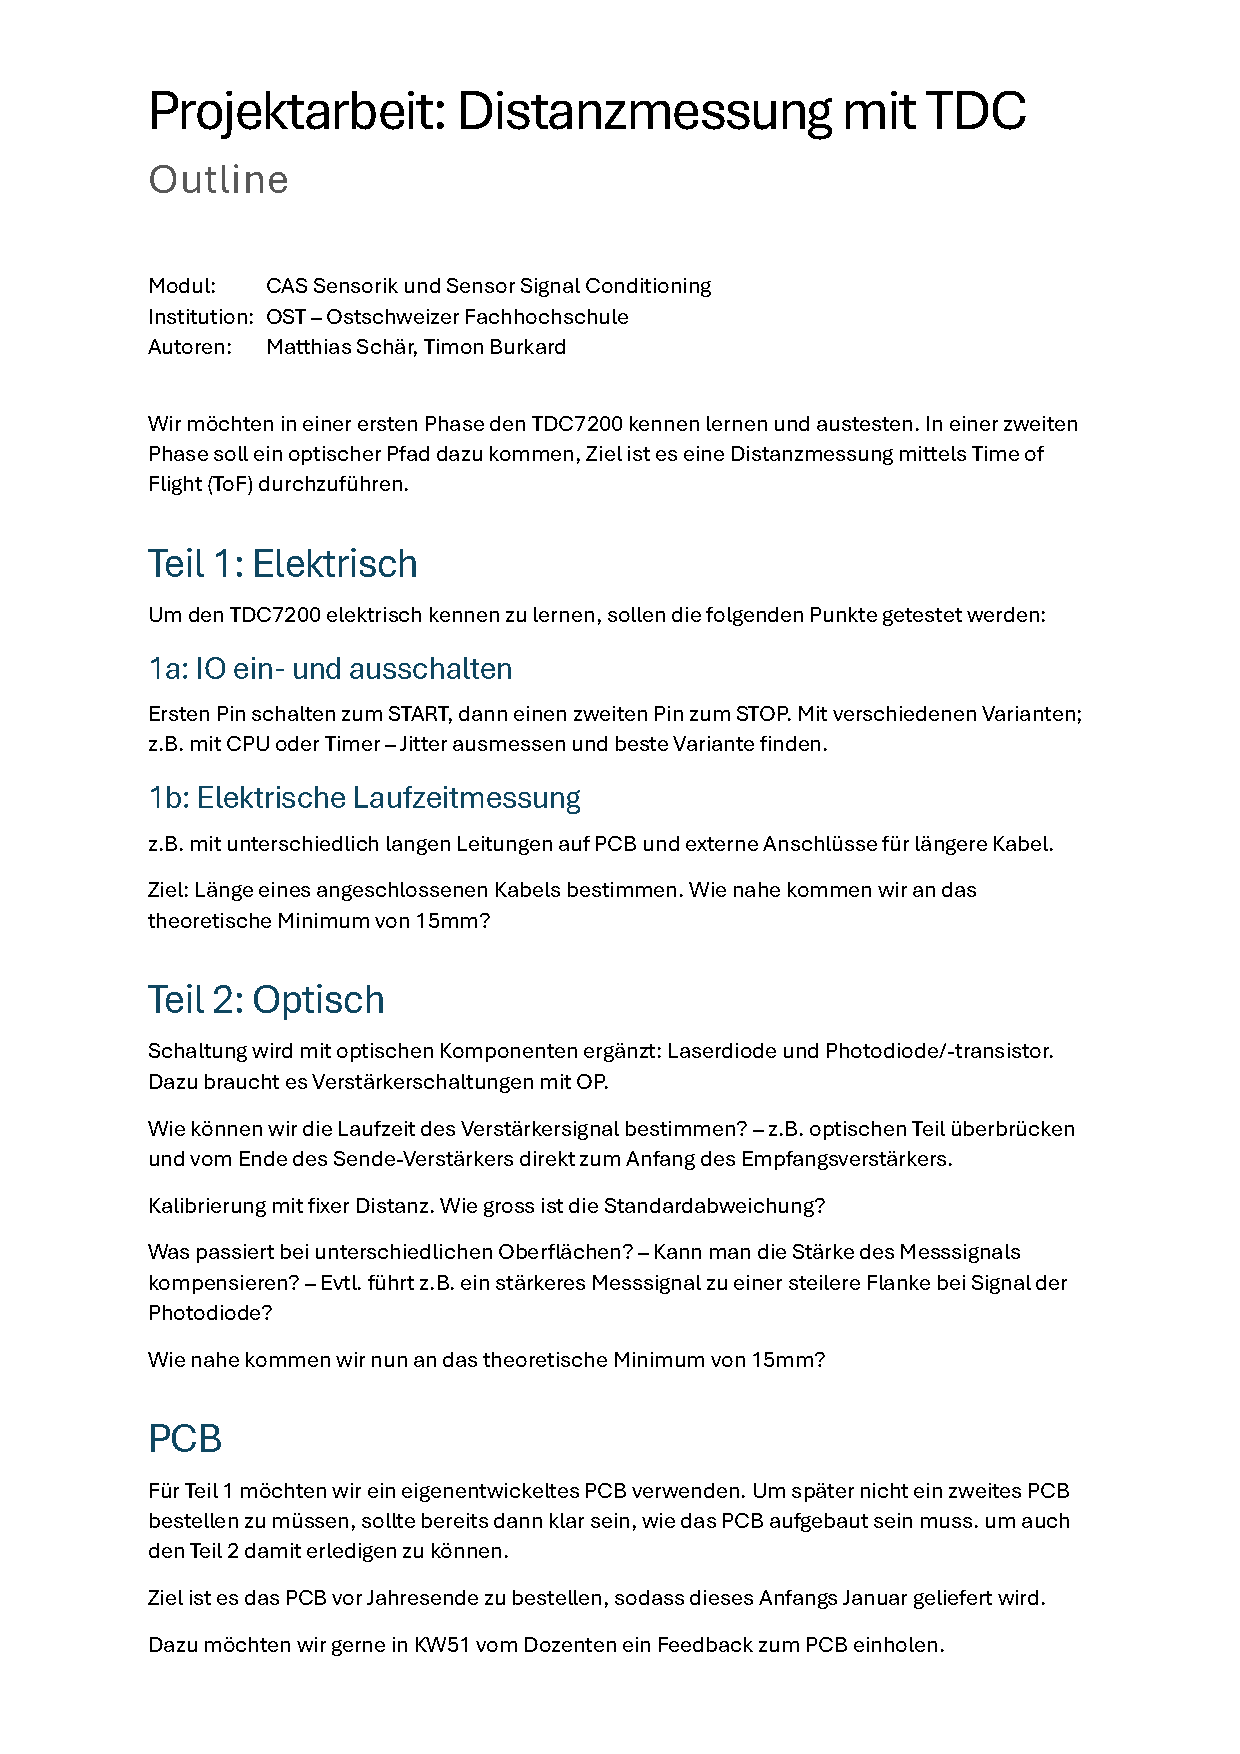
\includegraphics[page=1, width=0.89\textwidth, frame]{attachments/outline.pdf}
    \caption{Outline}\label{fig:outline}
\end{figure}

\subsection{TDC Treiber}\label{sec:tdc_driver}

In Code~\ref{code:tdc_driver_header} und \ref{code:tdc_driver_source} ist der selbst entwickelte Firmware-Treiber für
den \acrshort{tdc} dargestellt.

\lstinputlisting[language={c}, label={code:tdc_driver_header}, caption={\acrshort{tdc} Driver (Header)}]{../../firmware/Core/TDC/TDC.h}
\lstinputlisting[language={c}, label={code:tdc_driver_source}, caption={\acrshort{tdc} Driver (Source)}]{../../firmware/Core/TDC/TDC.c}

\subsection{Python Skripte}\label{sec:python_scripts}

In Code \ref{code:python_analyze} ist das Python-Skript zur Berechnung des arithmetischen Mittelwerts und der
Standardabweichung sowie zum Plotten des Histogramms und des Boxplots dargestellt.

\lstinputlisting[language={python}, label={code:python_analyze}, caption={Python Analyse}]{../../utilities/analyze-tof.py}

In Code \ref{code:python_analyze_multi_tofs} ist das Python-Skript zur Berechnung des arithmetischen Mittelwerts und der
Standardabweichung sowie zum Plotten der Werte für mehrere \acrshort{tof}-Datensätze dargestellt.

\lstinputlisting[language={python}, label={code:python_analyze_multi_tofs}, caption={Python Analyse (Multi \acrshort{tof}s)}]{../../utilities/analyze-tofs.py}

In Code \ref{code:python_analyze_multi_logs} ist das Python-Skript zum Plotten der Werte aus mehreren Log-Files
dargestellt.

\lstinputlisting[language={python}, label={code:python_analyze_multi_logs}, caption={Python Analyse (Multi Logs)}]{../../utilities/analyze-tofs-multi-logs.py}

In Code \ref{code:python_live_plot} ist das Python-Skript zum live Plotten von \acrshort{tof}-Werte dargestellt. Dieses
wird während der Präsentation für die Demonstration verwendet.

\lstinputlisting[language={python}, label={code:python_live_plot}, caption={Python Live Plot}]{../../utilities/live-plot.py}

\pagebreak

\begin{landscape}

    \subsection{Schema}\label{sec:schematic_apdx}
    \global\pdfpageattr\expandafter{\the\pdfpageattr/Rotate 90}
    \begin{figure}[H]
        \centering
        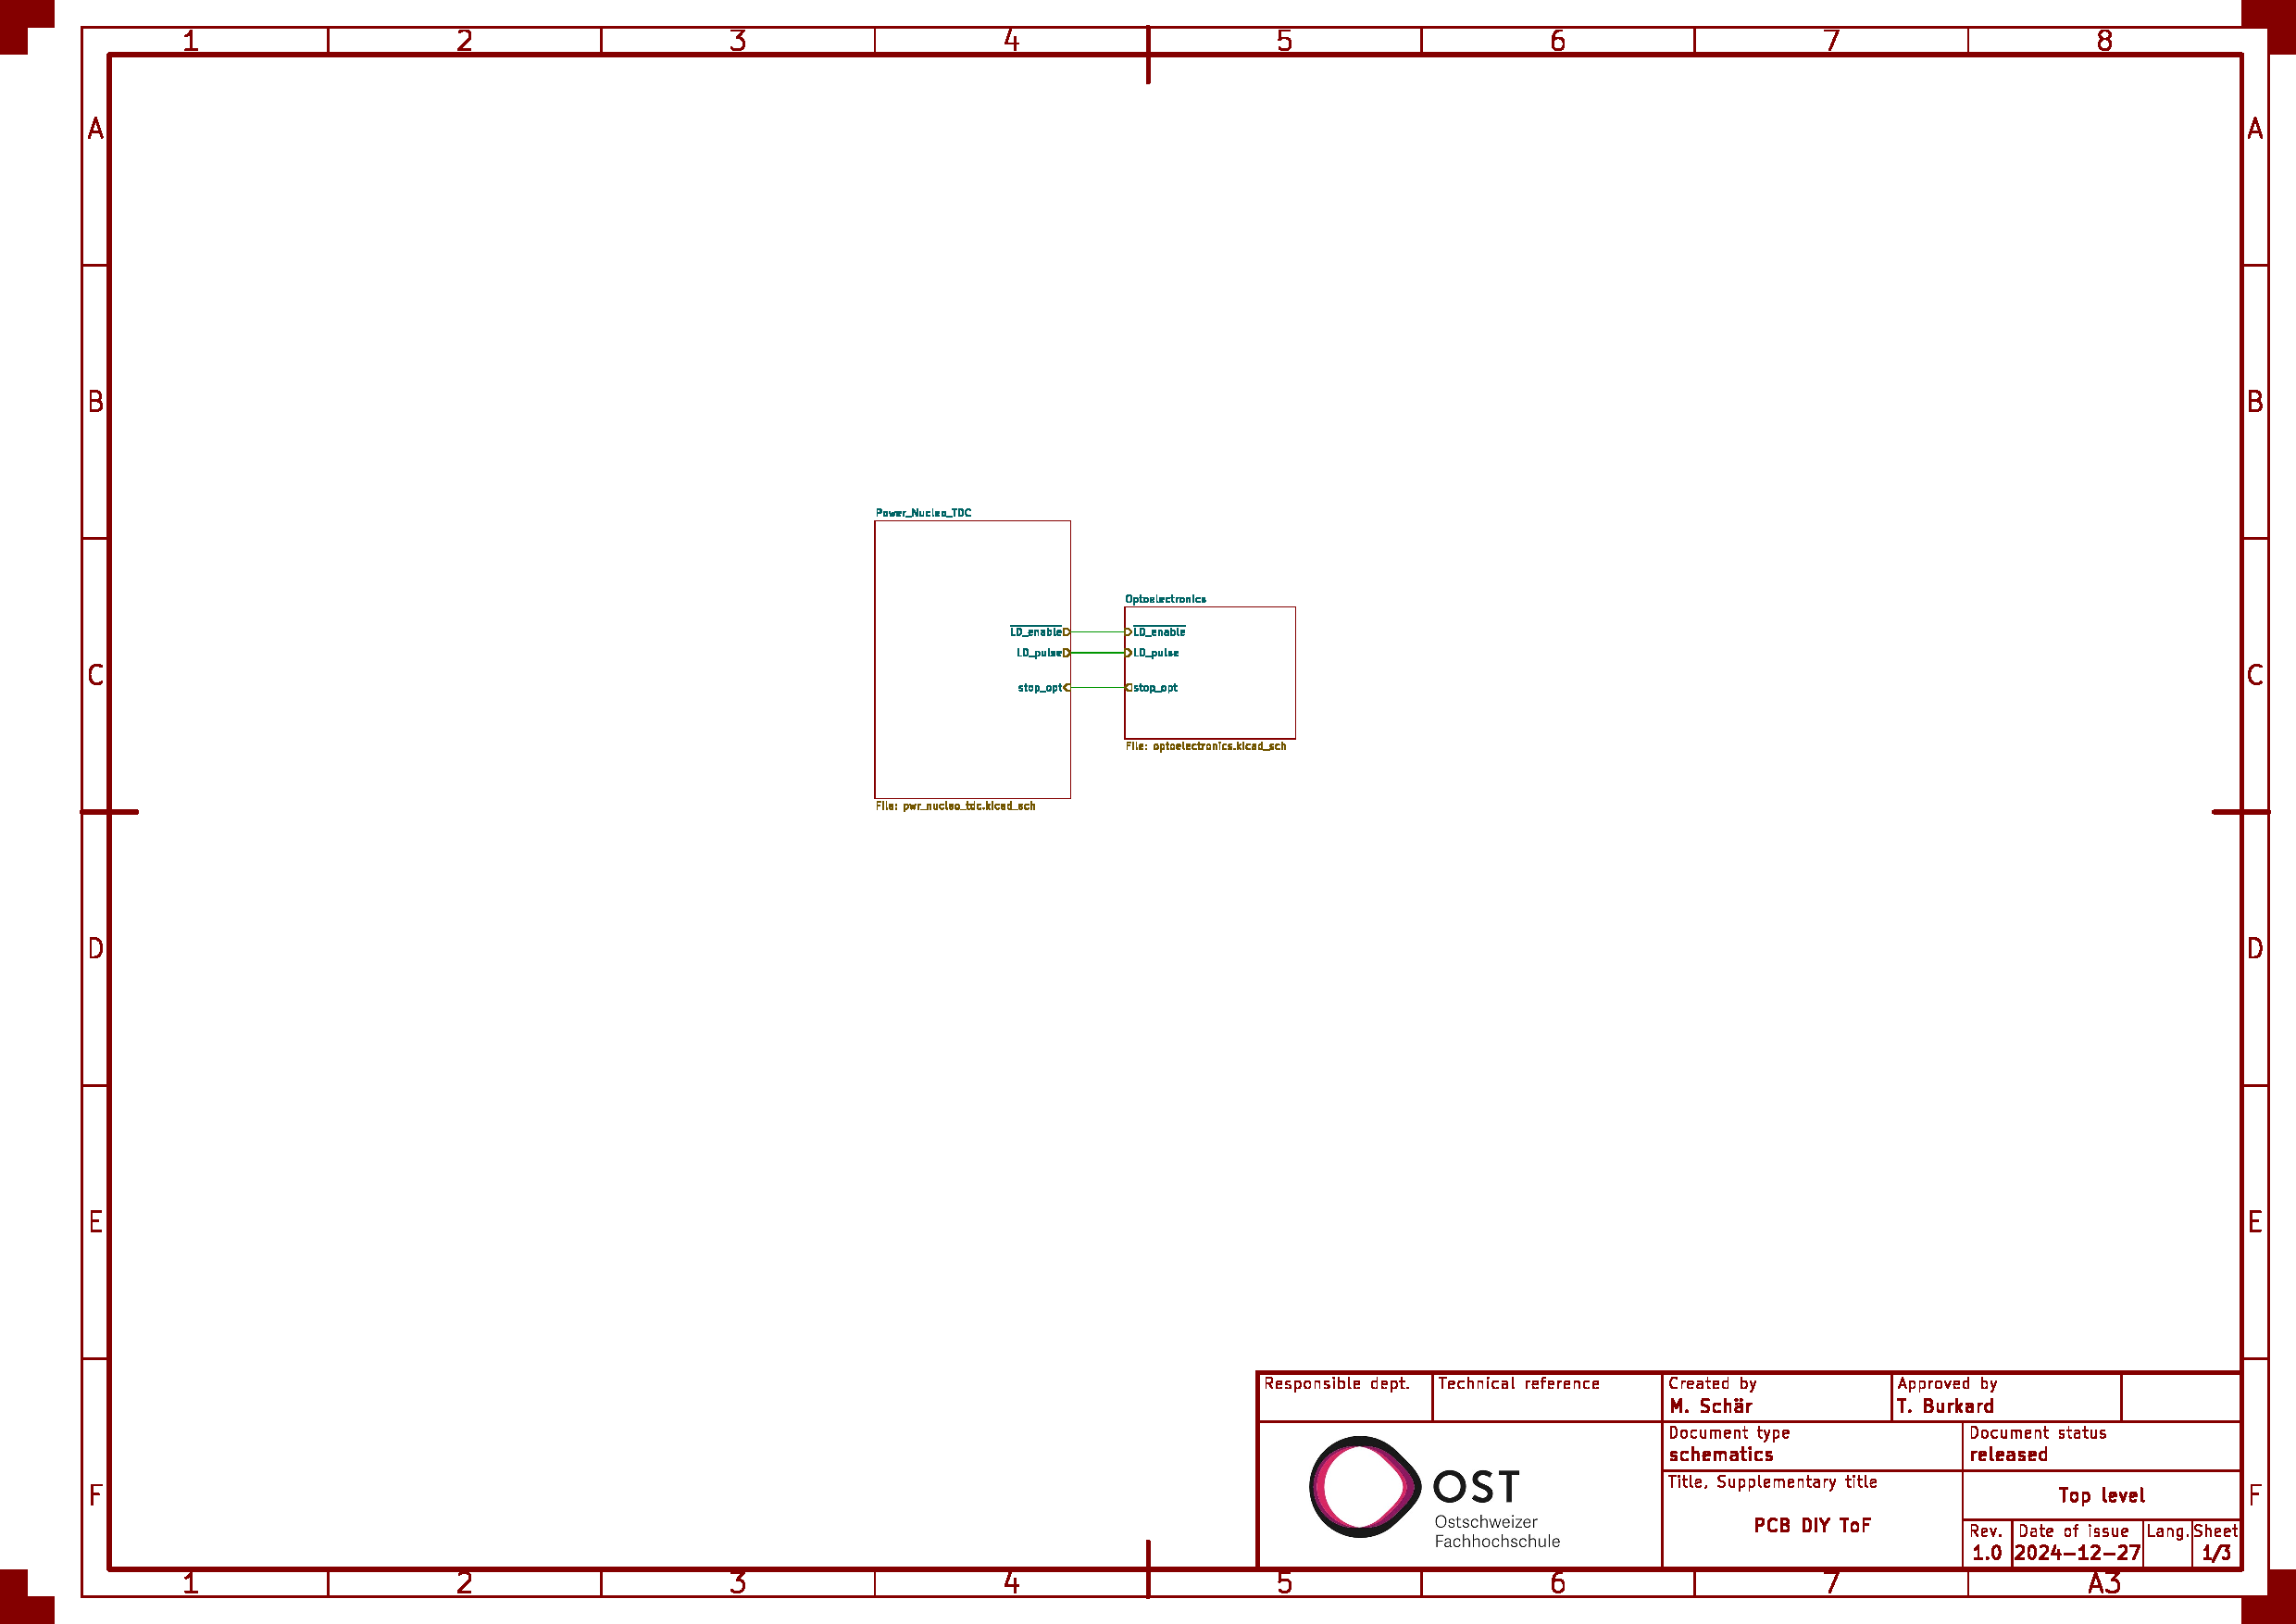
\includegraphics[page=1, width=1.2\textwidth]{attachments/schematic.pdf}
        \caption{Schema S.1/3}\label{fig:schematics_1}
    \end{figure}
    \pagebreak

    \global\pdfpageattr\expandafter{\the\pdfpageattr/Rotate 90}
    \begin{figure}[H]
        \centering
        \includegraphics[page=2, width=1.2\textwidth]{attachments/schematic.pdf}
        \caption{Schema S.2/3}\label{fig:schematics_2}
    \end{figure}
    \pagebreak

    \global\pdfpageattr\expandafter{\the\pdfpageattr/Rotate 90}
    \begin{figure}[H]
        \centering
        \includegraphics[page=3, width=1.2\textwidth]{attachments/schematic.pdf}
        \caption{Schema S.3/3}\label{fig:schematics_3}
    \end{figure}
    \pagebreak

    \subsection{Stückliste}

    \begin{table}[H]
        \scriptsize
        \mytable
            {|l|l|l|l|l|l|}
            {\textbf{Reference} & \textbf{Value} & \textbf{Datasheet} & \textbf{Footprint} & \textbf{Qty} & \textbf{DNP}}
            {\Reference & \Value & \Datasheet & \Footprint & \Qty & \DNP}
            {tables/bom.csv}
        \caption{Bill of Material}\label{tab:bom}
    \end{table}

\end{landscape}
\global\pdfpageattr\expandafter{\the\pdfpageattr/Rotate 0}

\subsection{Layout}\label{sec:apdx_layout}

\begin{figure}[H]
    \centering
    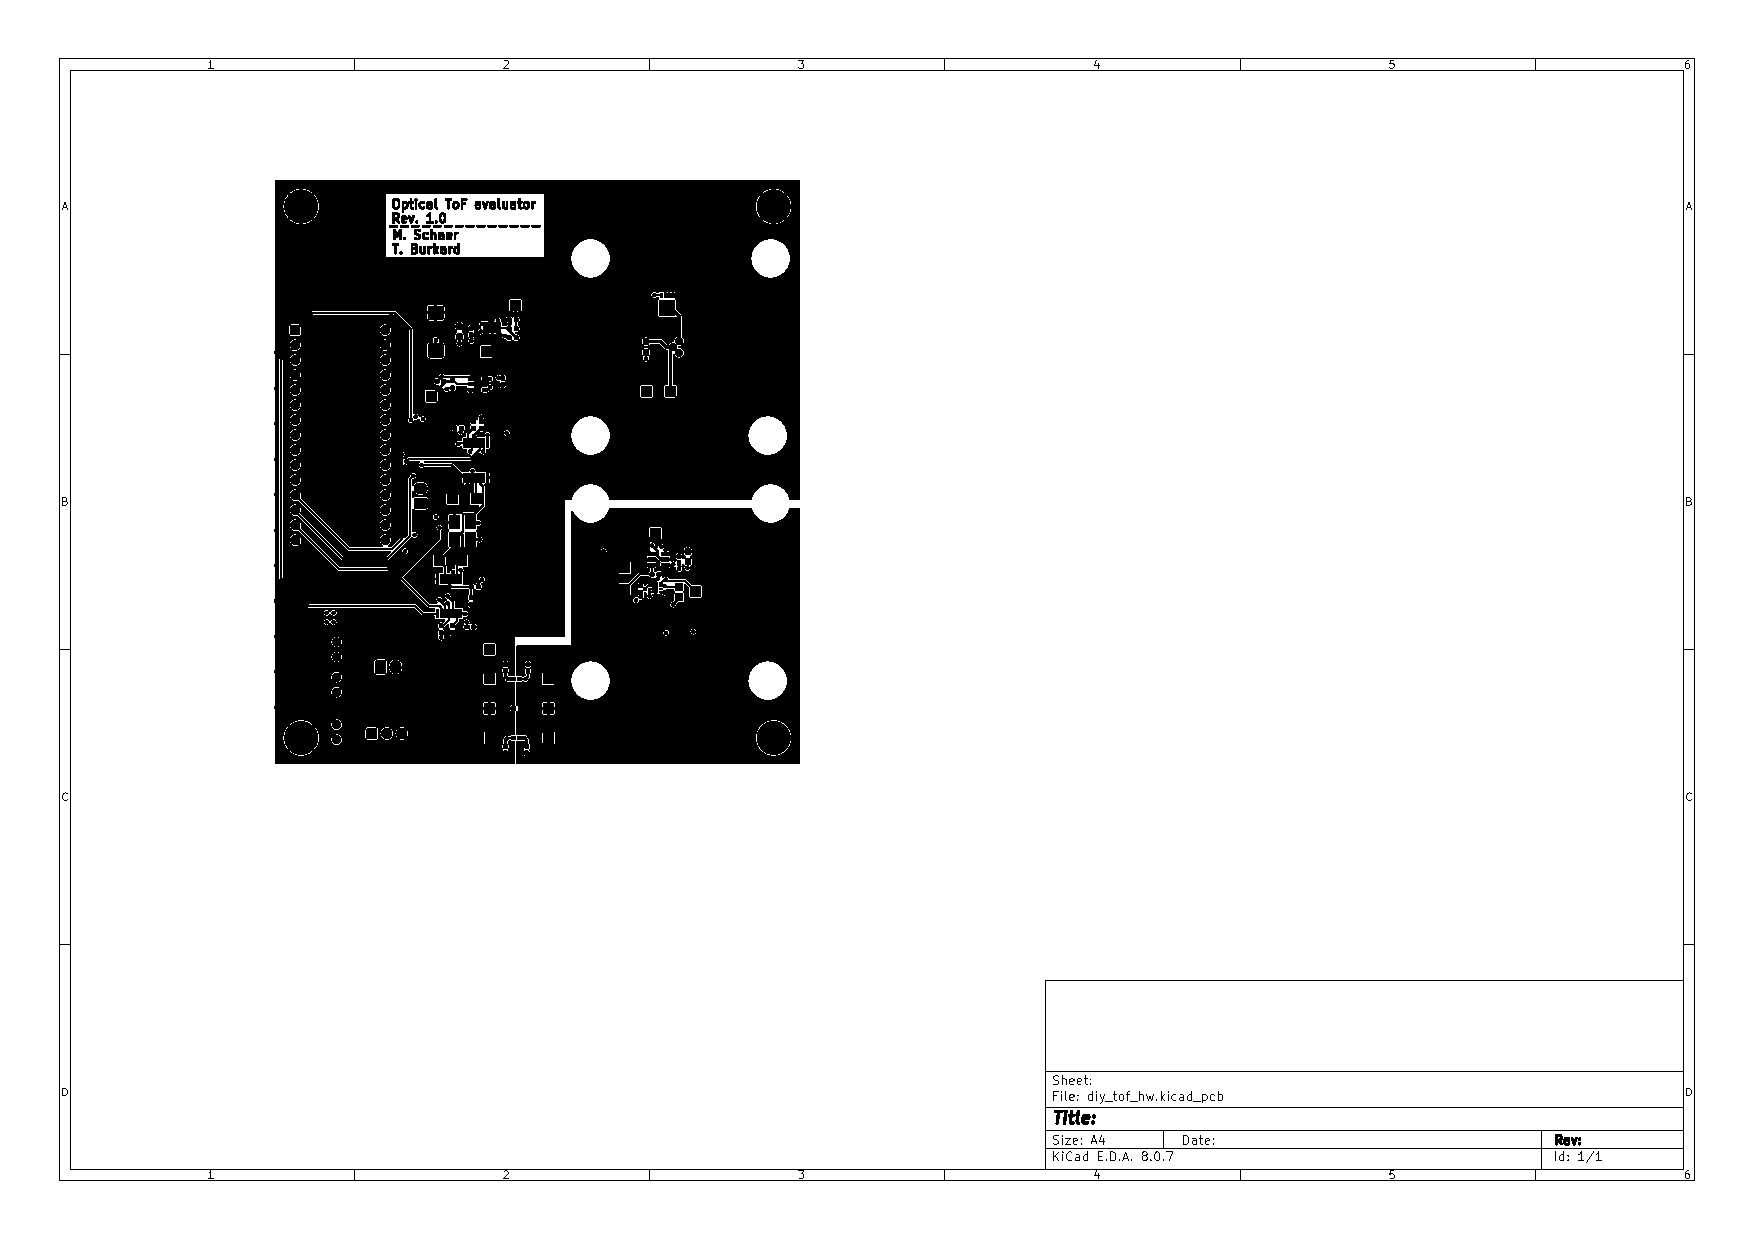
\includegraphics[trim=130 220 450 80, clip, width=0.6\textwidth]{attachments/pcb_F_Cu.pdf}
    \caption{PCB Layout Top}\label{fig:apdx_pcb_f_cu}
\end{figure}

\begin{figure}[H]
    \centering
    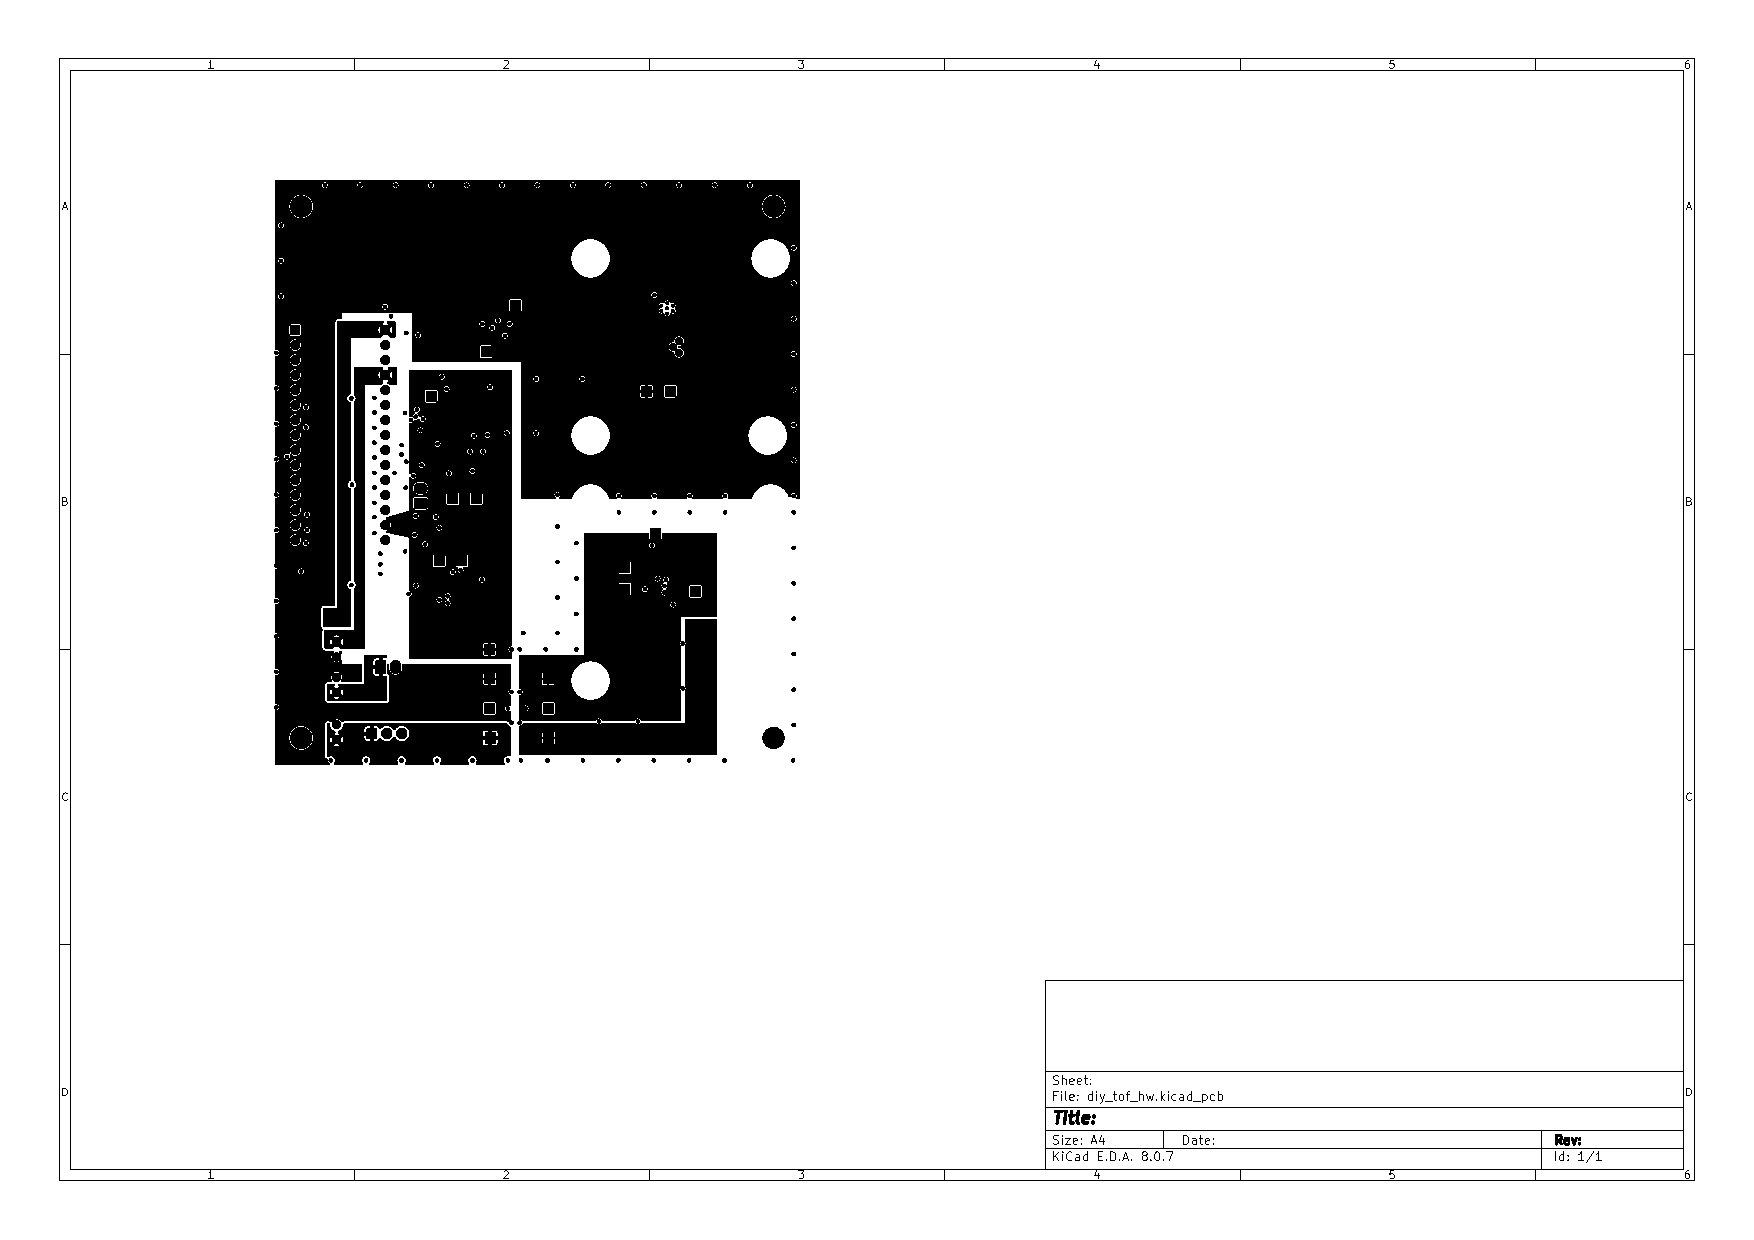
\includegraphics[trim=130 220 450 80, clip, width=0.6\textwidth]{attachments/pcb_In1_Cu.pdf}
    \caption{PCB Layout Innen 1}\label{fig:apdx_pcb_in1_cu}
\end{figure}

\begin{figure}[H]
    \centering
    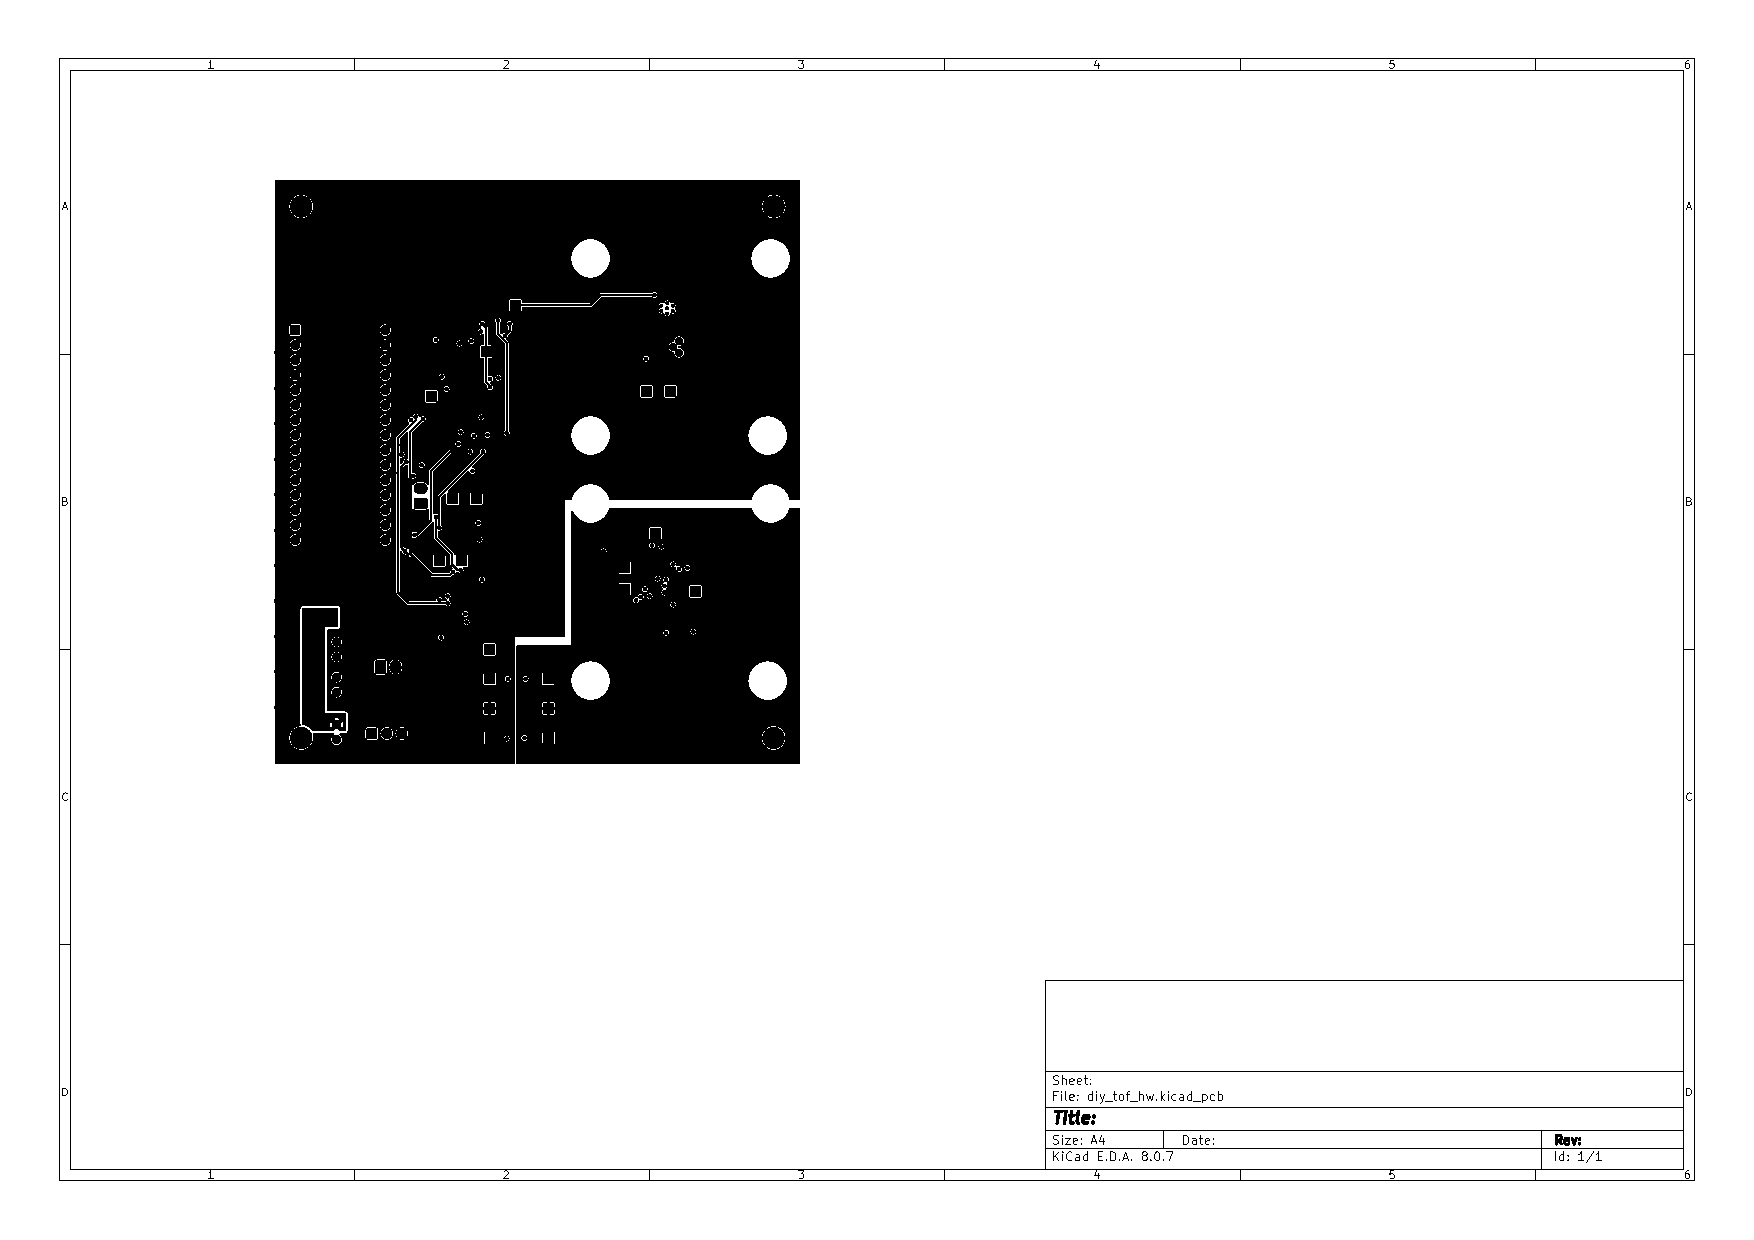
\includegraphics[trim=130 220 450 80, clip, width=0.6\textwidth]{attachments/pcb_In2_Cu.pdf}
    \caption{PCB Layout Innen 2}\label{fig:apdx_pcb_in2_cu}
\end{figure}

\begin{figure}[H]
    \centering
    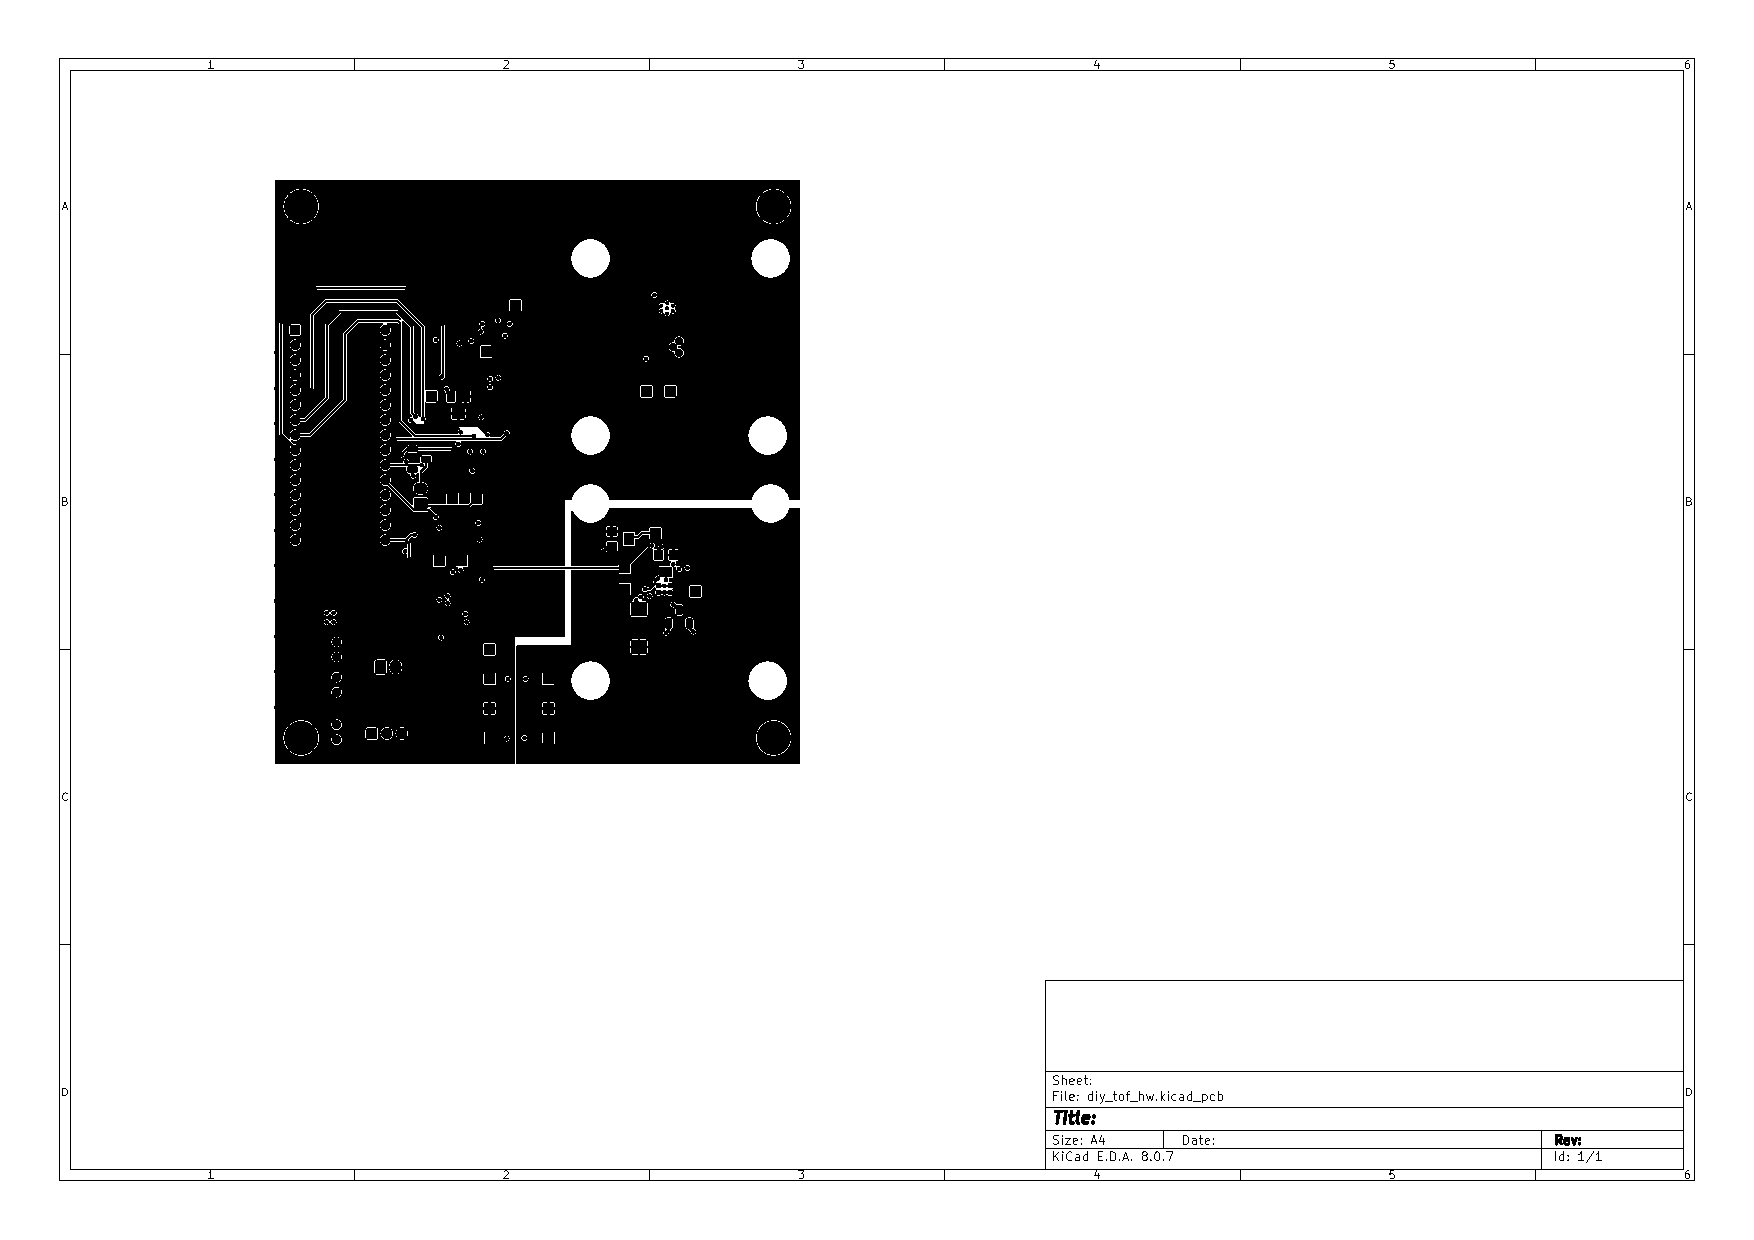
\includegraphics[trim=130 220 450 80, clip, width=0.6\textwidth]{attachments/pcb_B_Cu.pdf}
    \caption{PCB Layout Bottom}\label{fig:apdx_pcb_b_cu}
\end{figure}

\subsection{Komponenten-Platzierung}\label{sec:apdx_placement}

\begin{figure}[H]
    \centering
    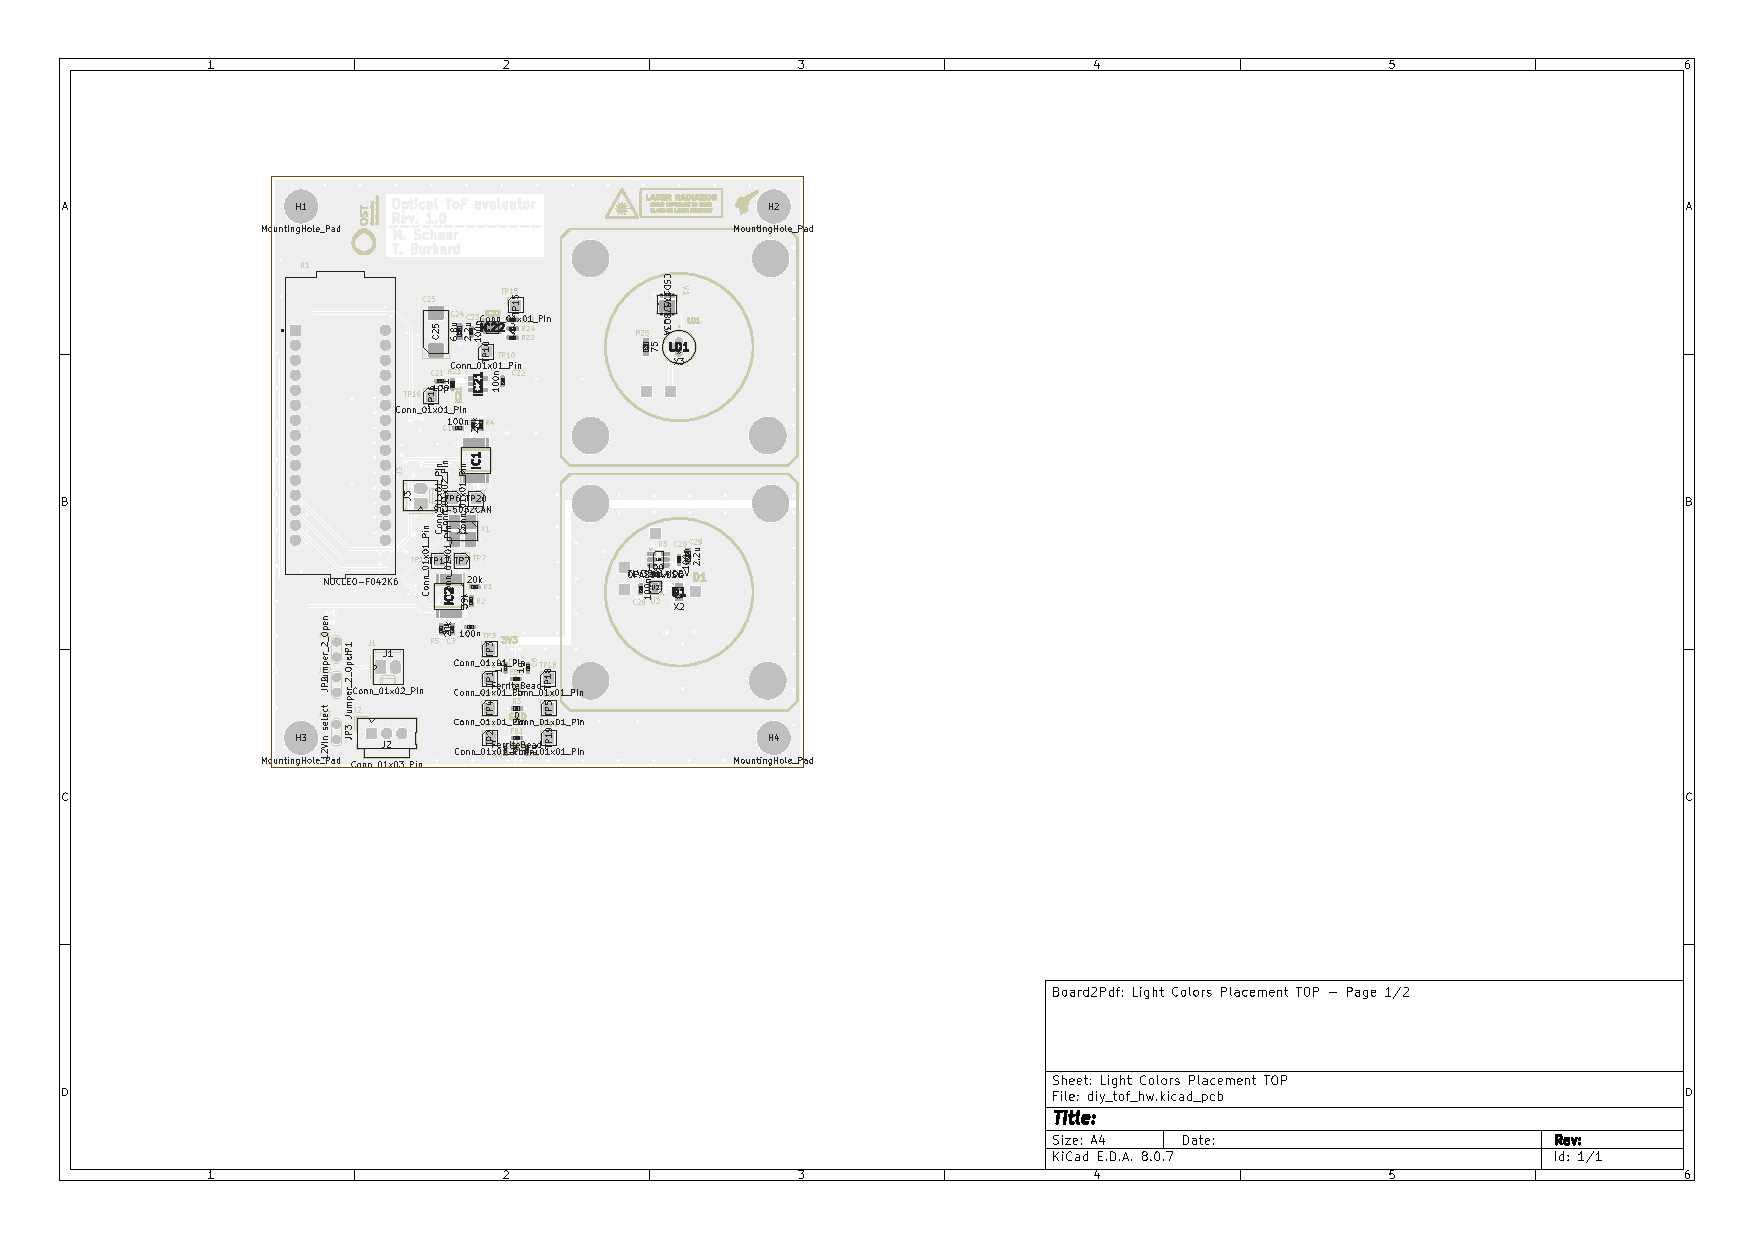
\includegraphics[page=1, trim=120 220 450 80, clip, width=0.6\textwidth]{attachments/pcb_placement.pdf}
    \caption{PCB Komponenten-Platzierung Top}\label{fig:apdx_pcb_placement_1}
\end{figure}

\begin{figure}[H]
    \centering
    \includegraphics[page=2, trim=450 220 120 80, clip, width=0.6\textwidth]{attachments/pcb_placement.pdf}
    \caption{PCB Komponenten-Platzierung Bottom}\label{fig:apdx_pcb_placement_2}
\end{figure}
\pagebreak

\subsection{3D View}\label{sec:apdx_3D_view}

\begin{figure}[H]
    \centering
    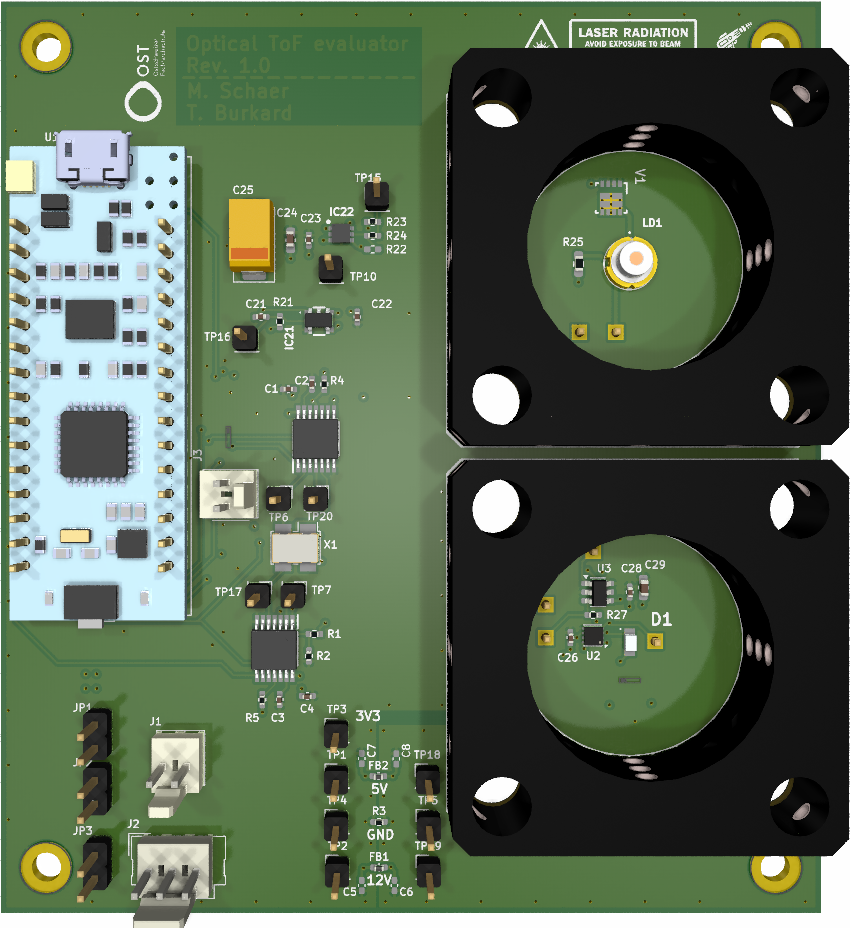
\includegraphics[width=0.55\textwidth]{graphics/3d_top.png}
    \caption{3D View Top}\label{fig:apdx_3d_top}
\end{figure}

\begin{figure}[H]
    \centering
    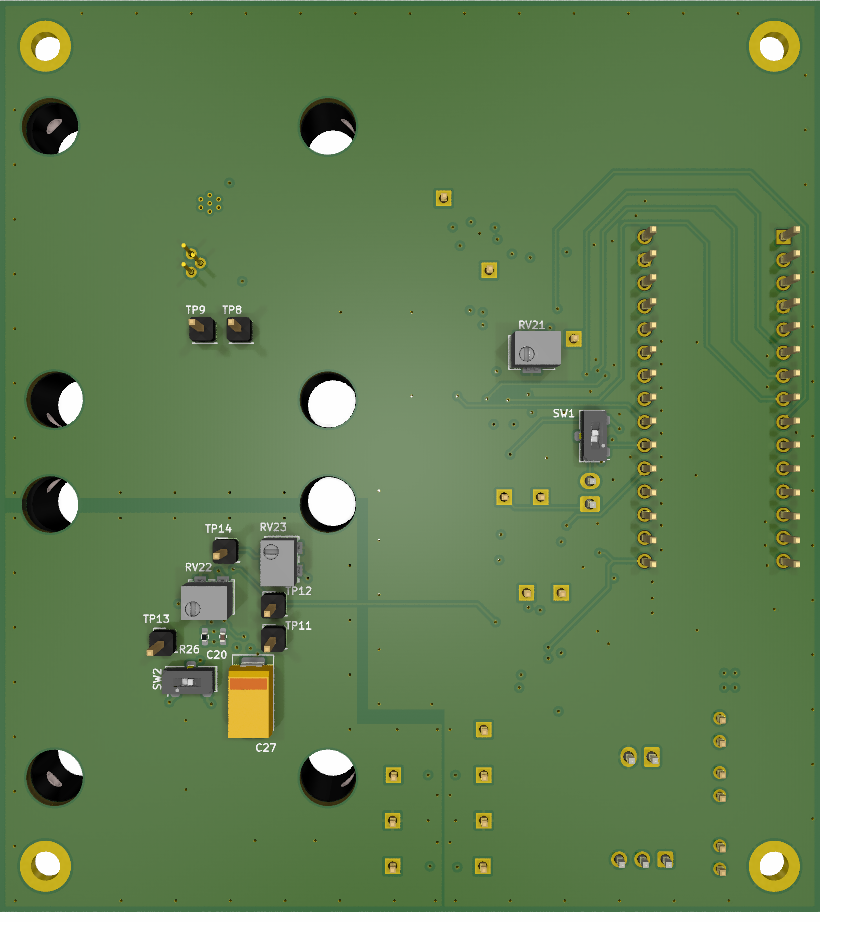
\includegraphics[width=0.55\textwidth]{graphics/3d_bottom.png}
    \caption{3D View Bottom}\label{fig:apdx_3d_bottom}
\end{figure}

\subsection{Fotos Demonstrator}\label{sec:apdx_photos_demonstrator}

\begin{figure}[H]
    \centering
    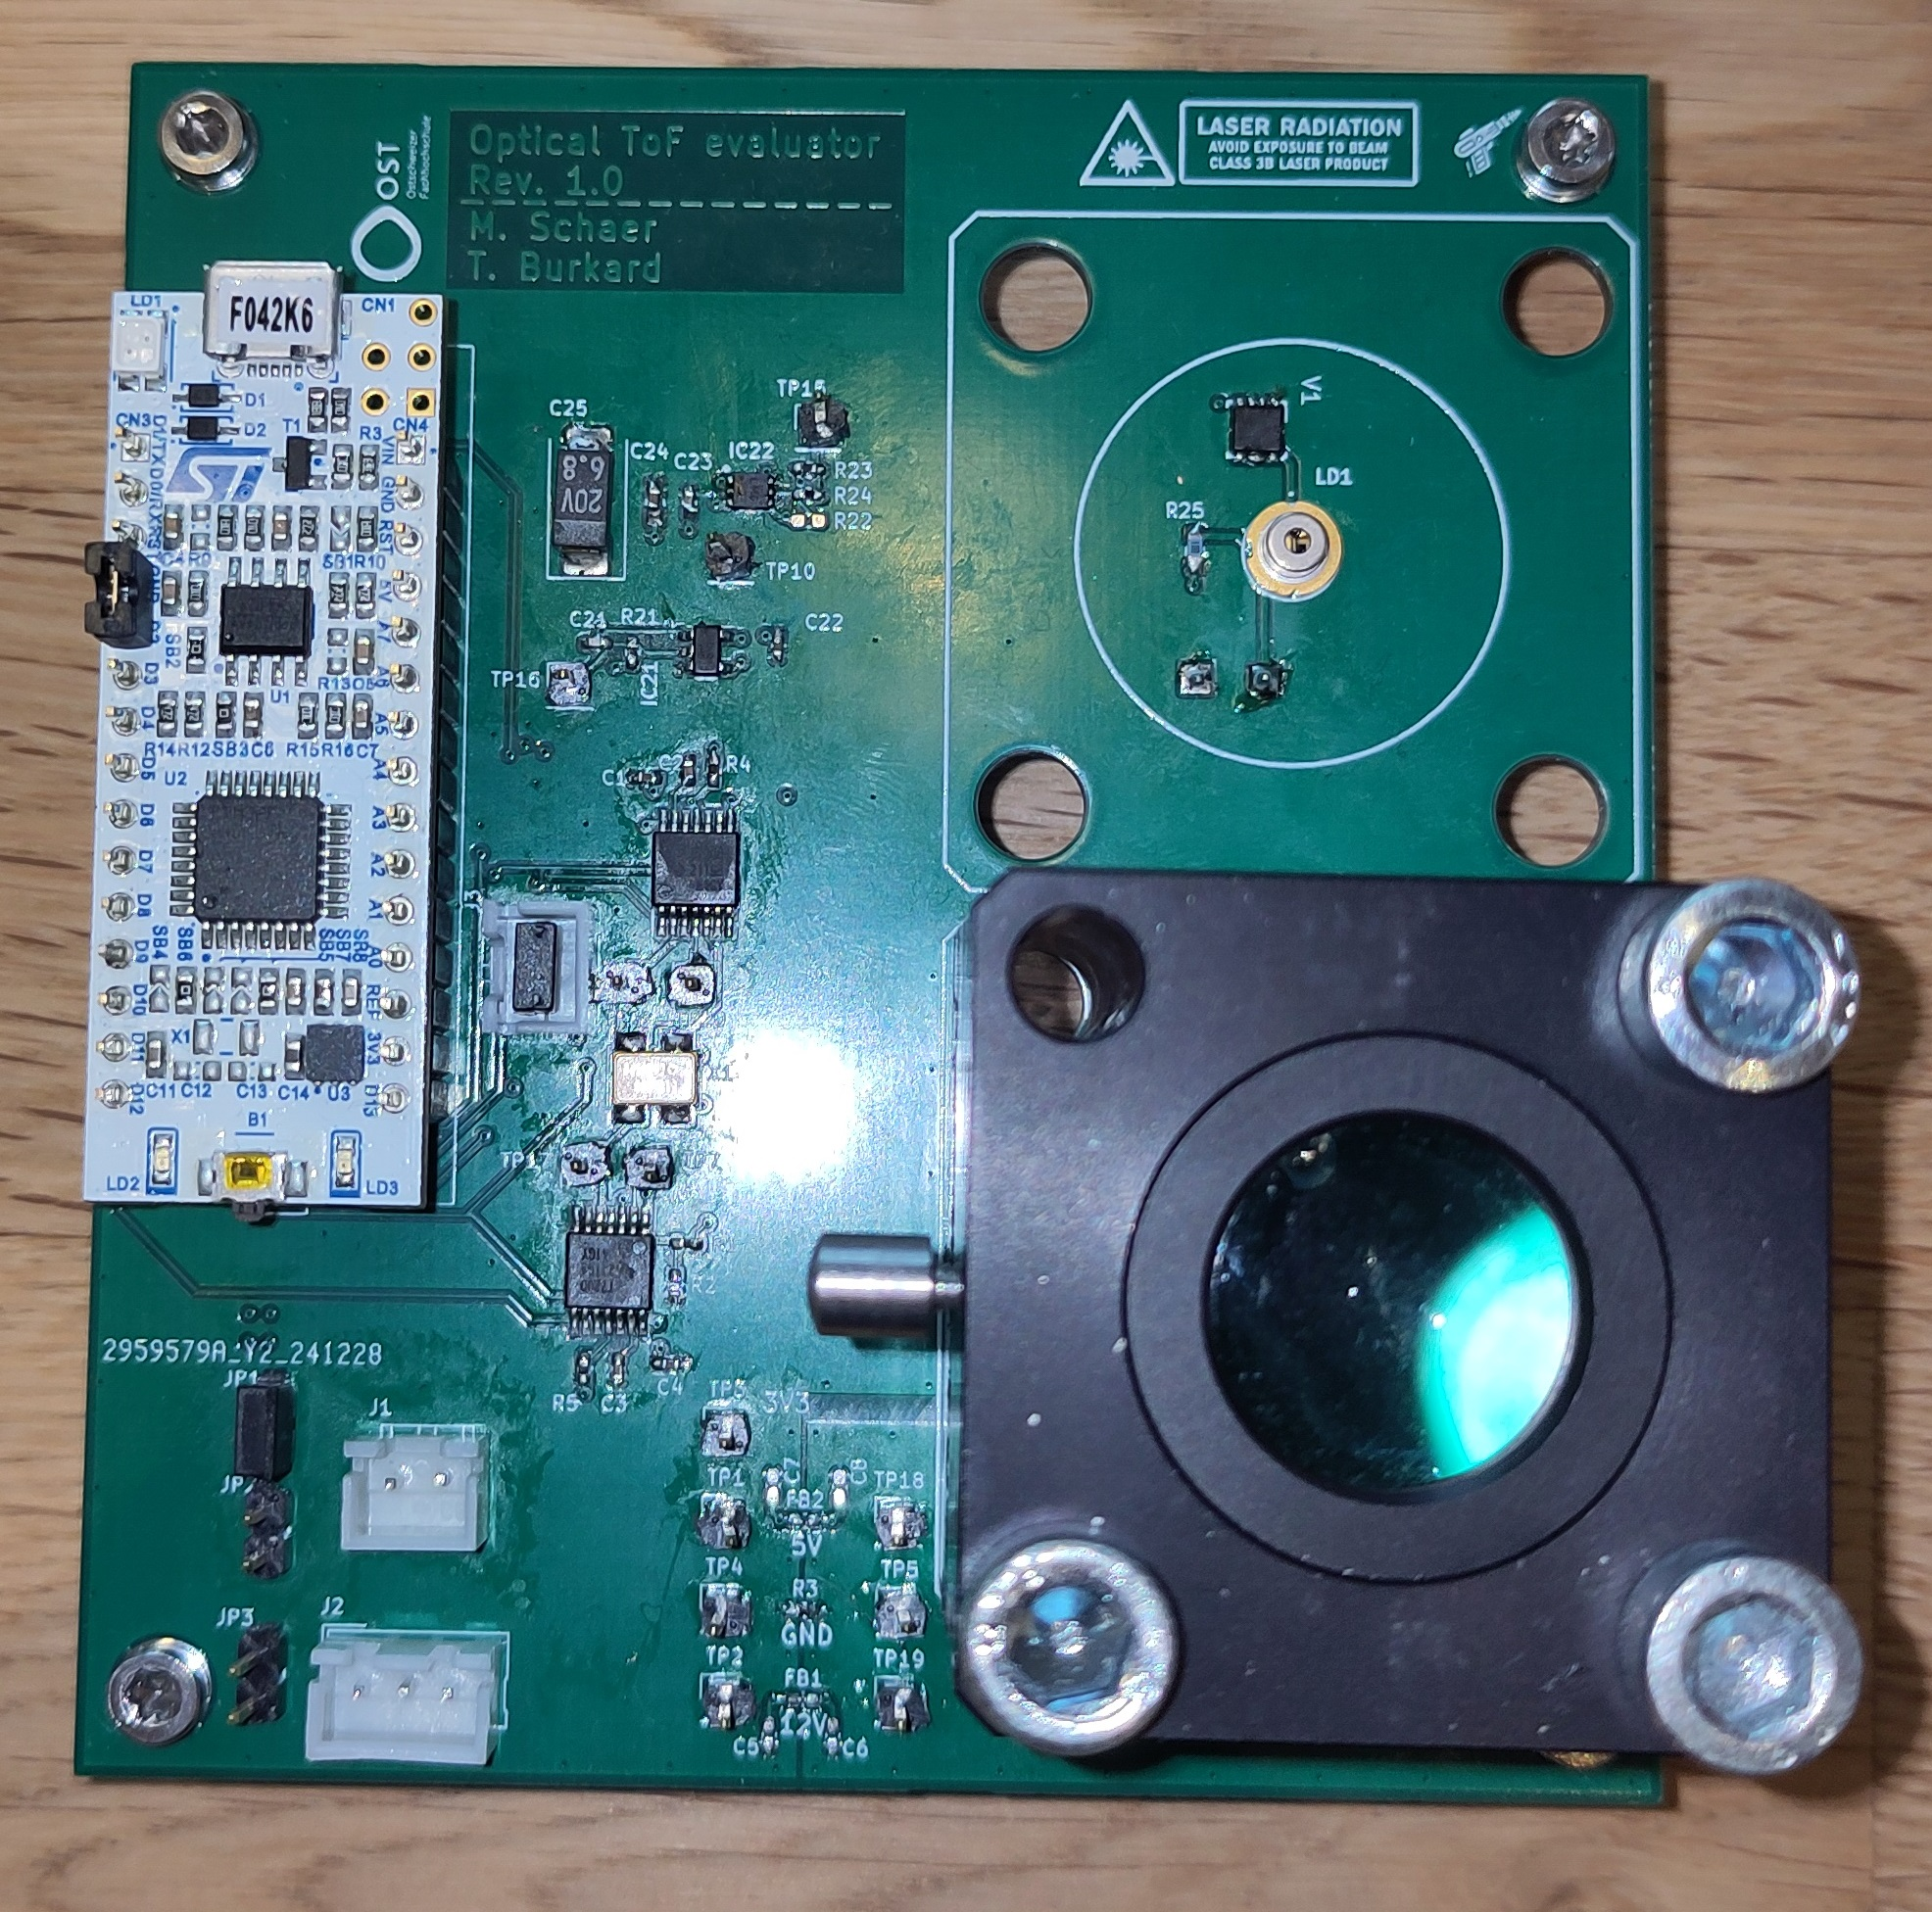
\includegraphics[width=0.6\textwidth]{graphics/photo_demonstrator_top.jpg}
    \caption{Demonstrator von oben}\label{fig:apdx_photo_demonstrator_top}
\end{figure}

\begin{figure}[H]
    \centering
    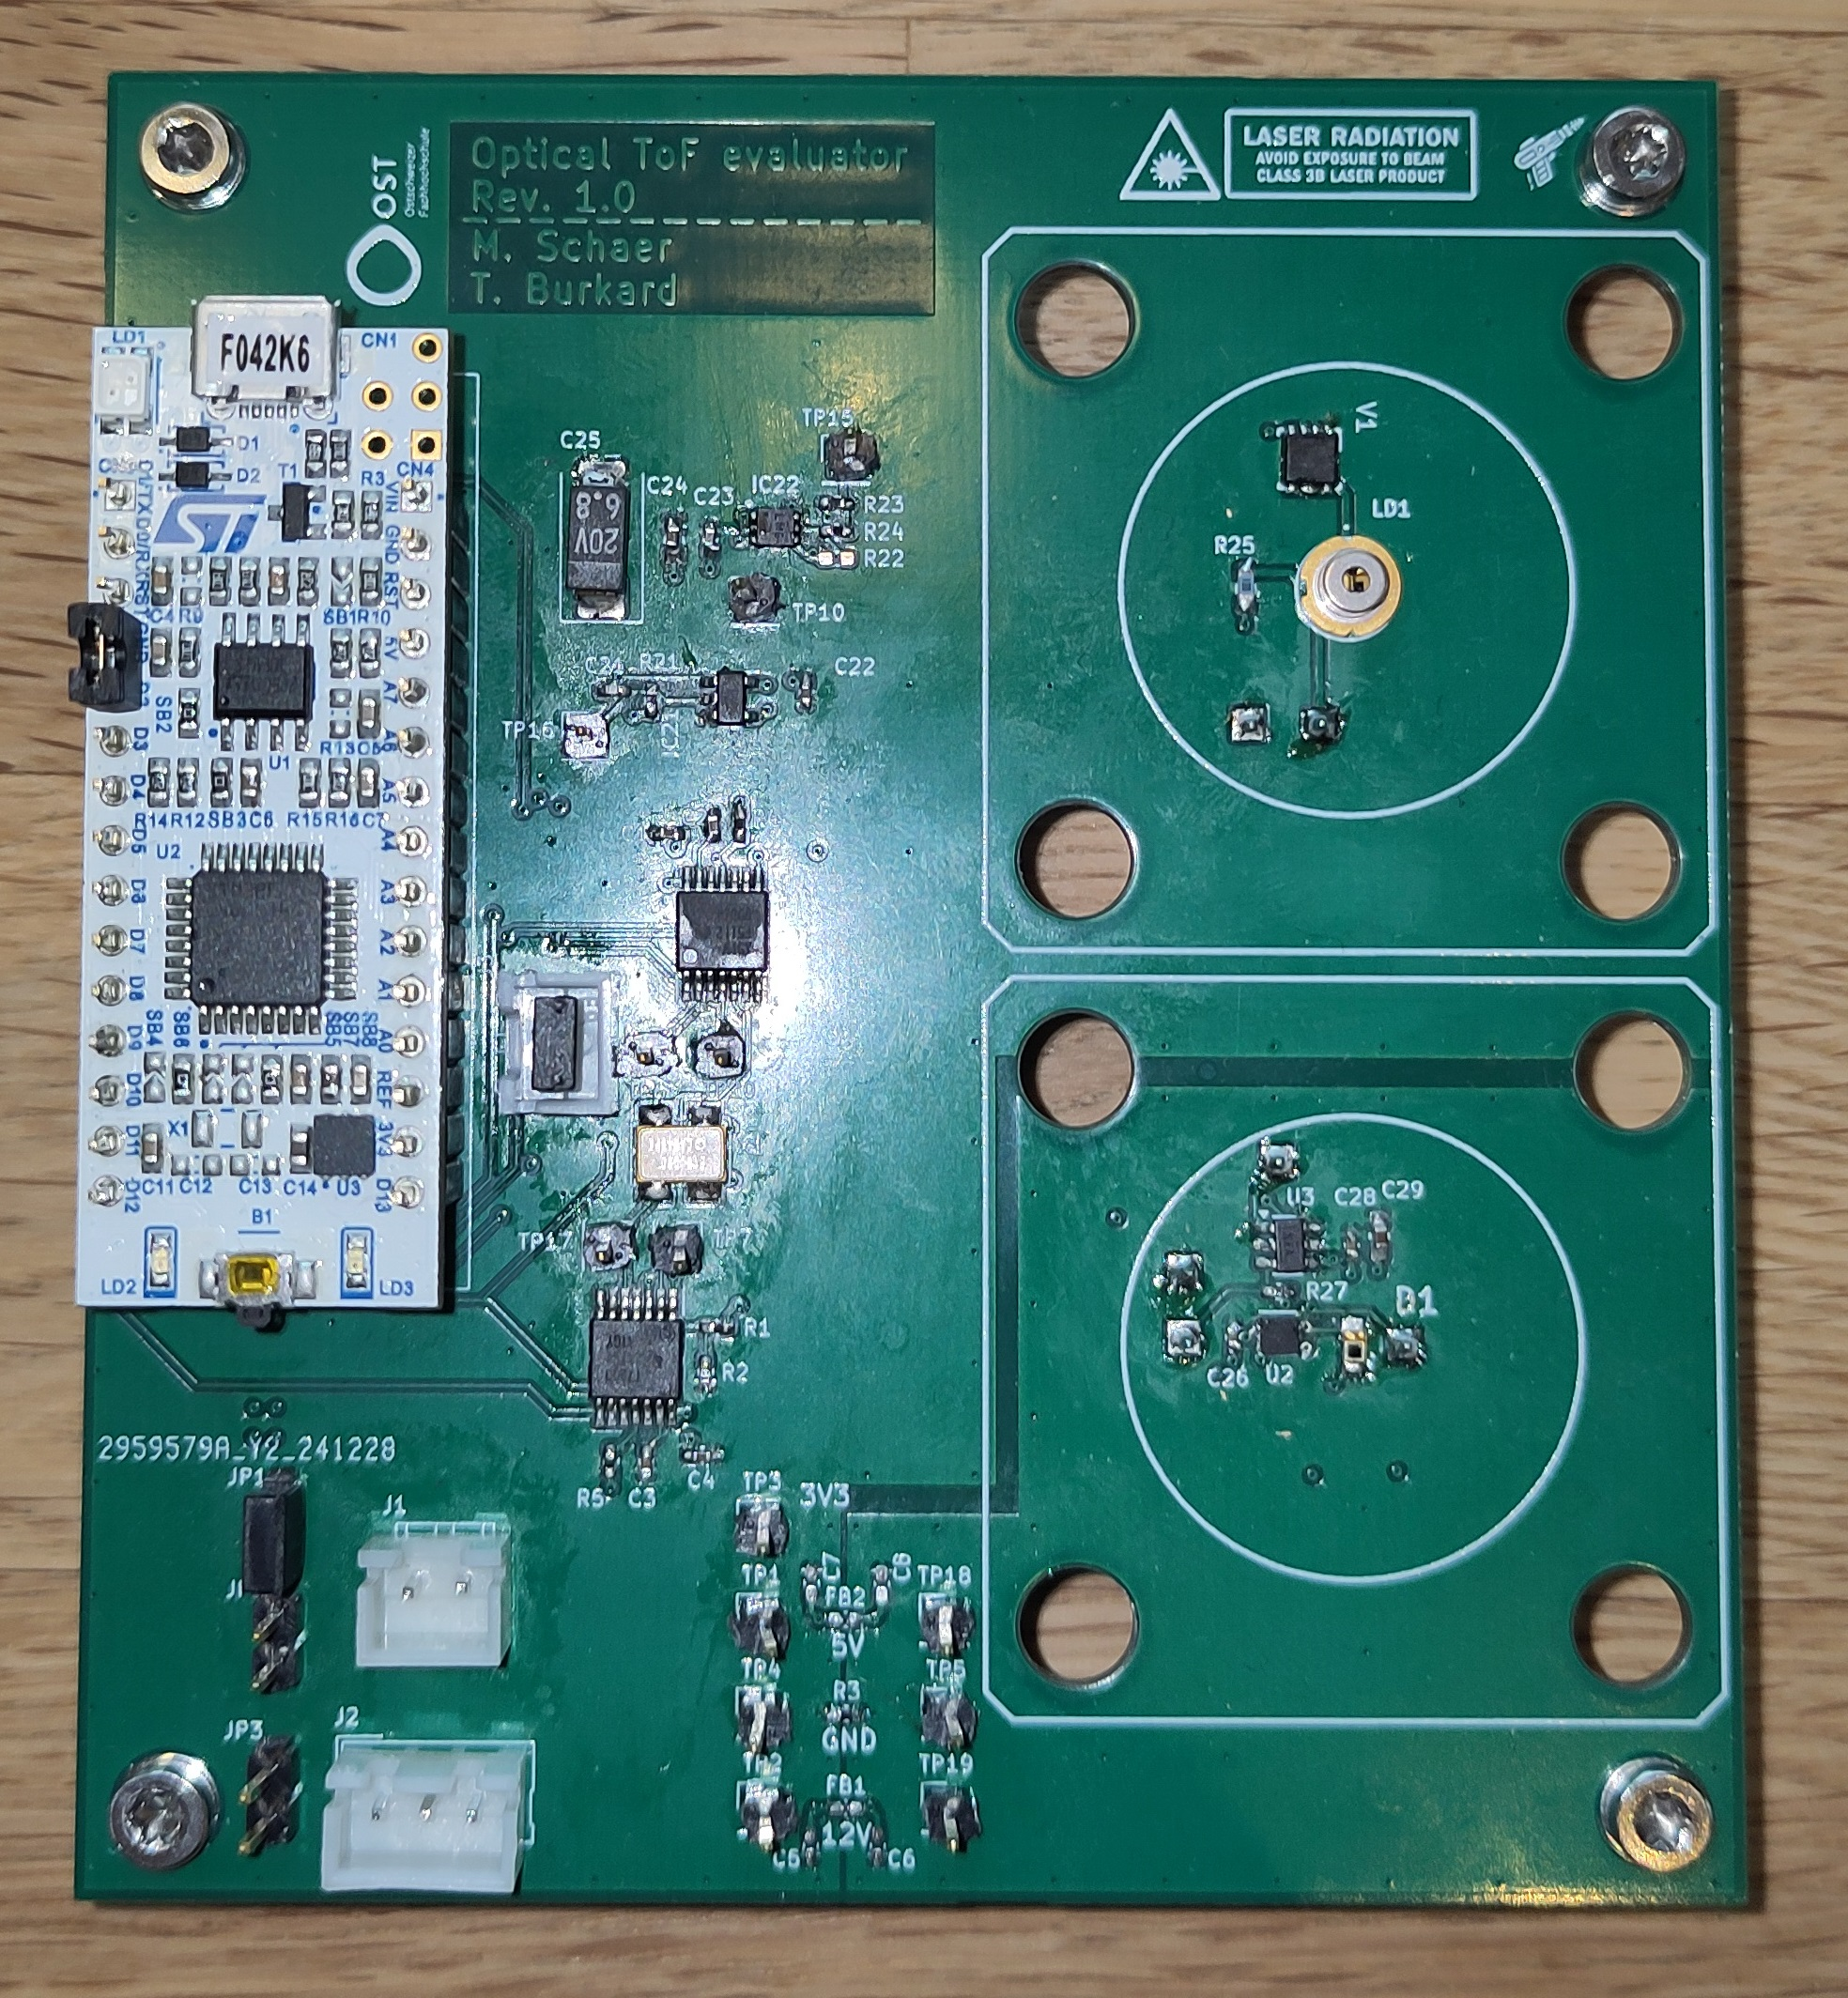
\includegraphics[width=0.6\textwidth]{graphics/photo_demonstrator_top_wo_lens.jpg}
    \caption{Demonstrator von oben ohne Linse}\label{fig:apdx_photo_demonstrator_top_wo_lens}
\end{figure}

\begin{figure}[H]
    \centering
    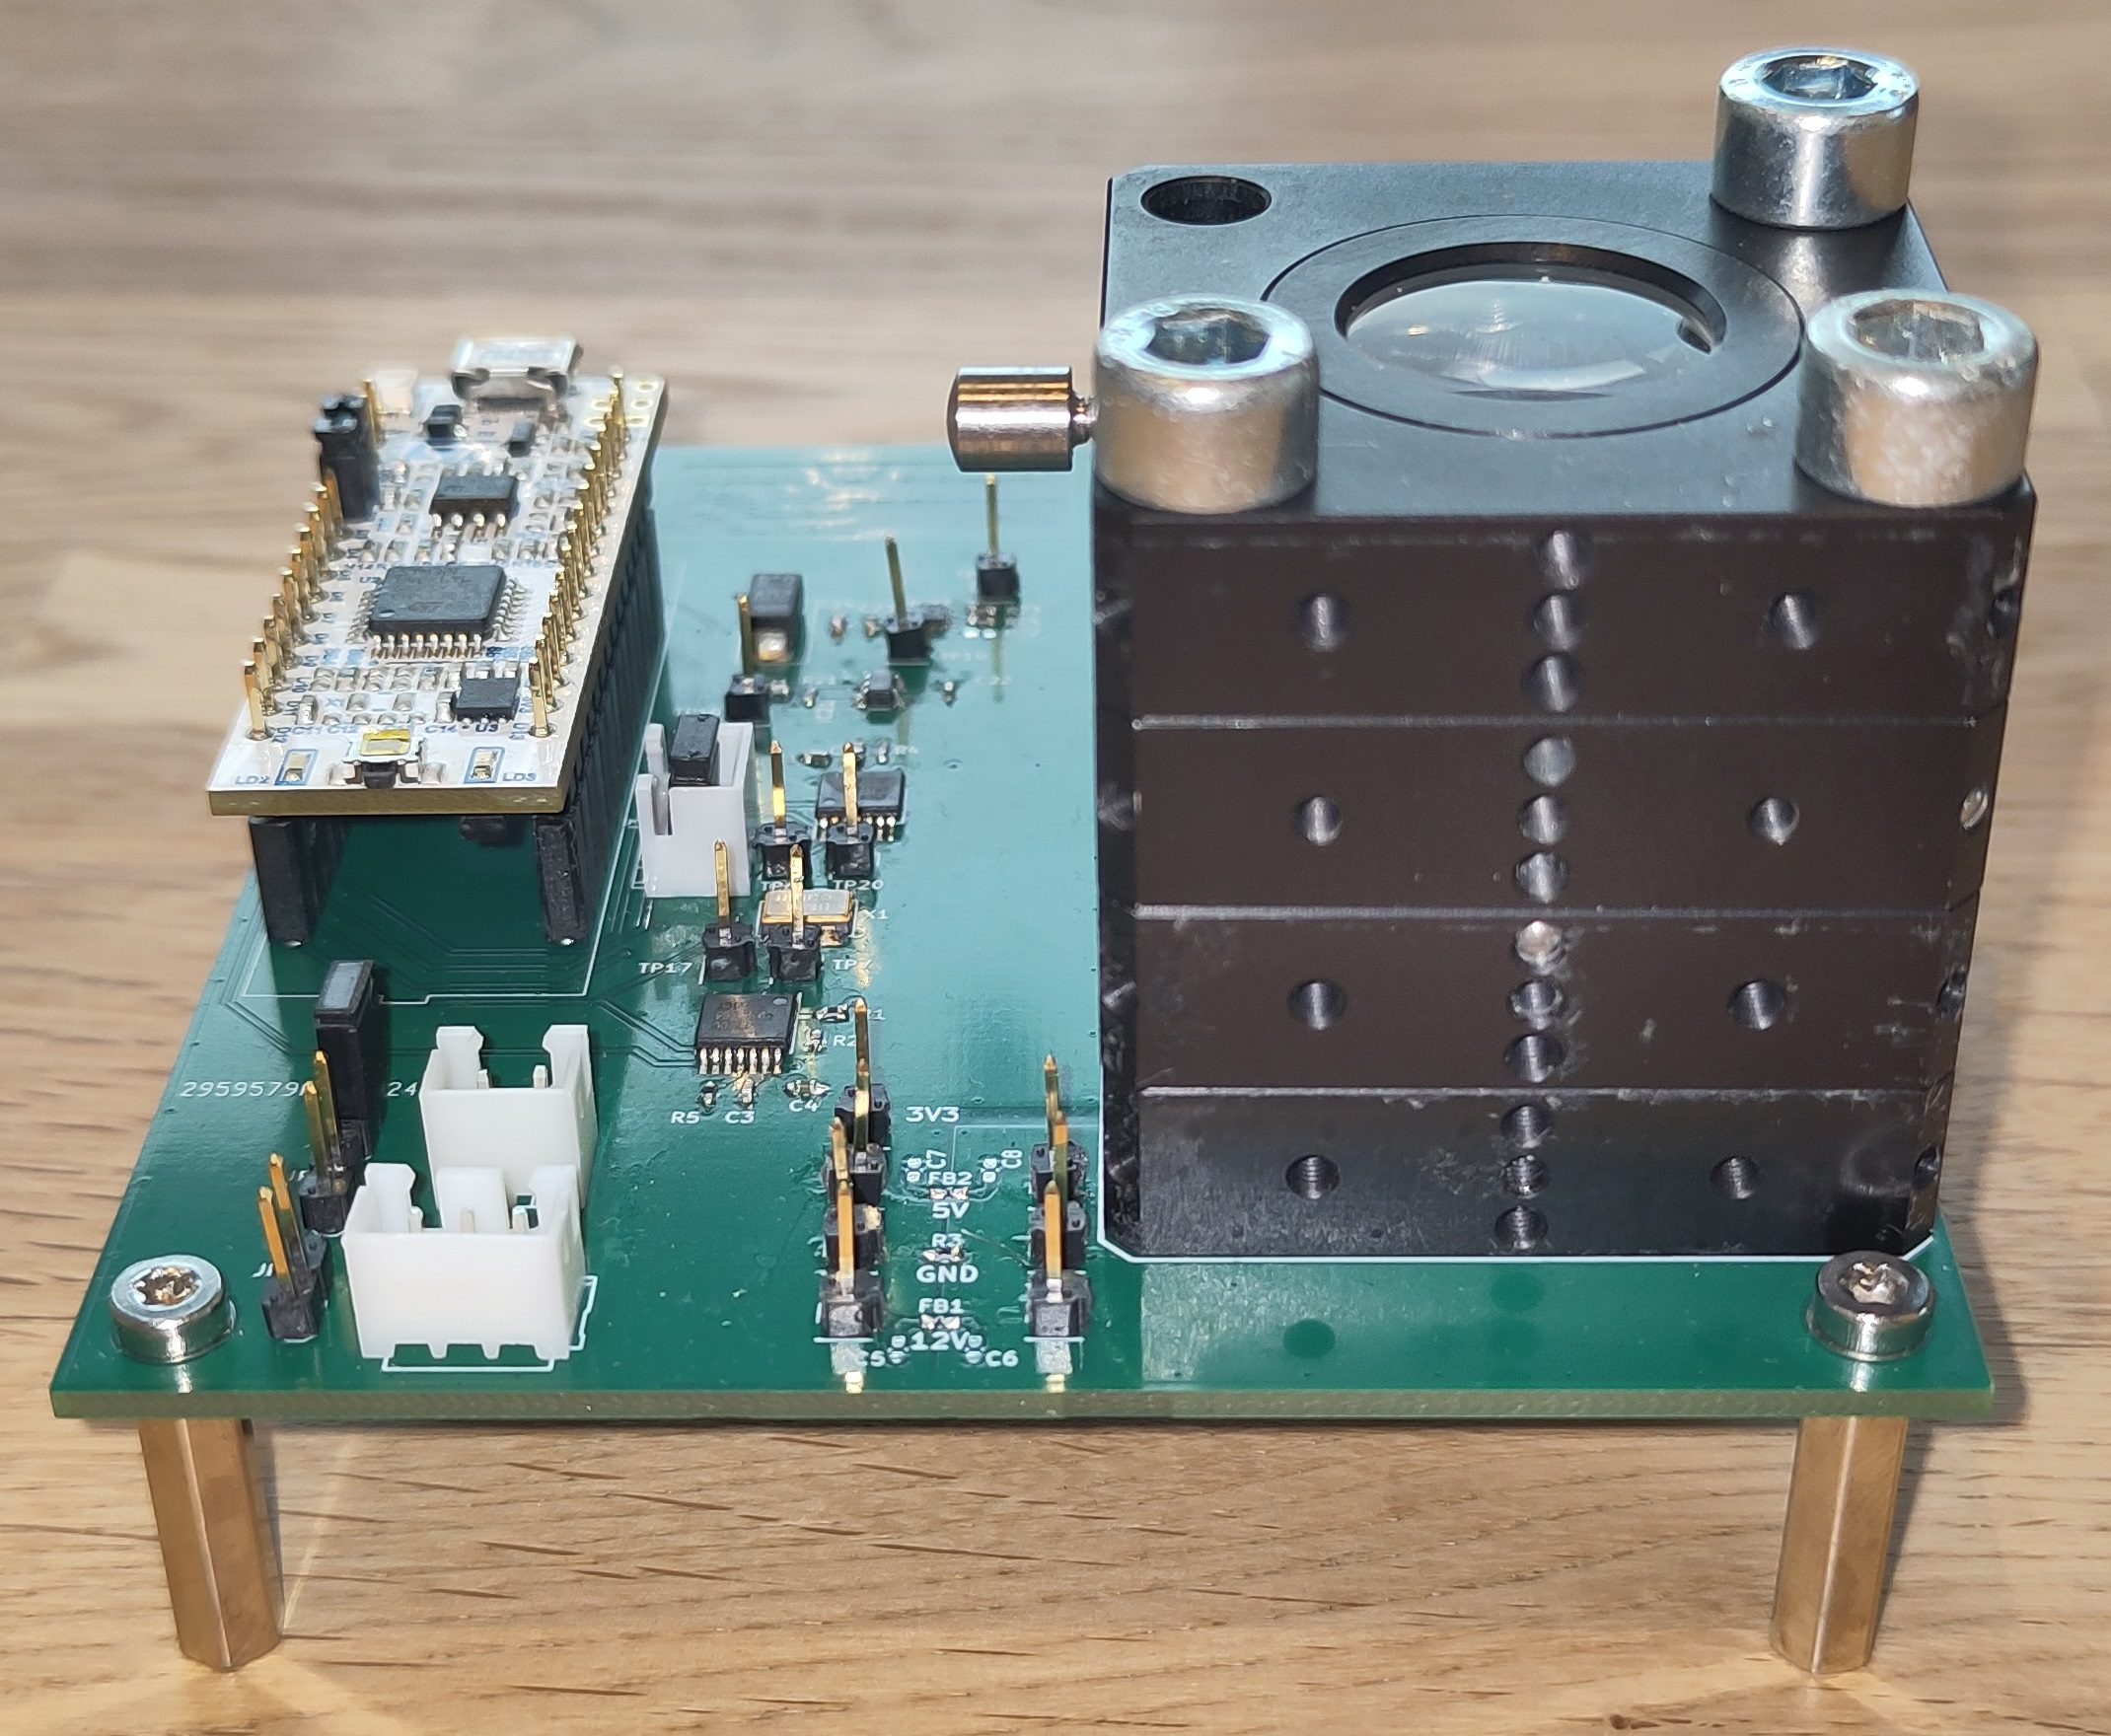
\includegraphics[width=0.6\textwidth]{graphics/photo_demonstrator_front.jpg}
    \caption{Demonstrator von vorne}\label{fig:apdx_photo_demonstrator_front}
\end{figure}

\begin{figure}[H]
    \centering
    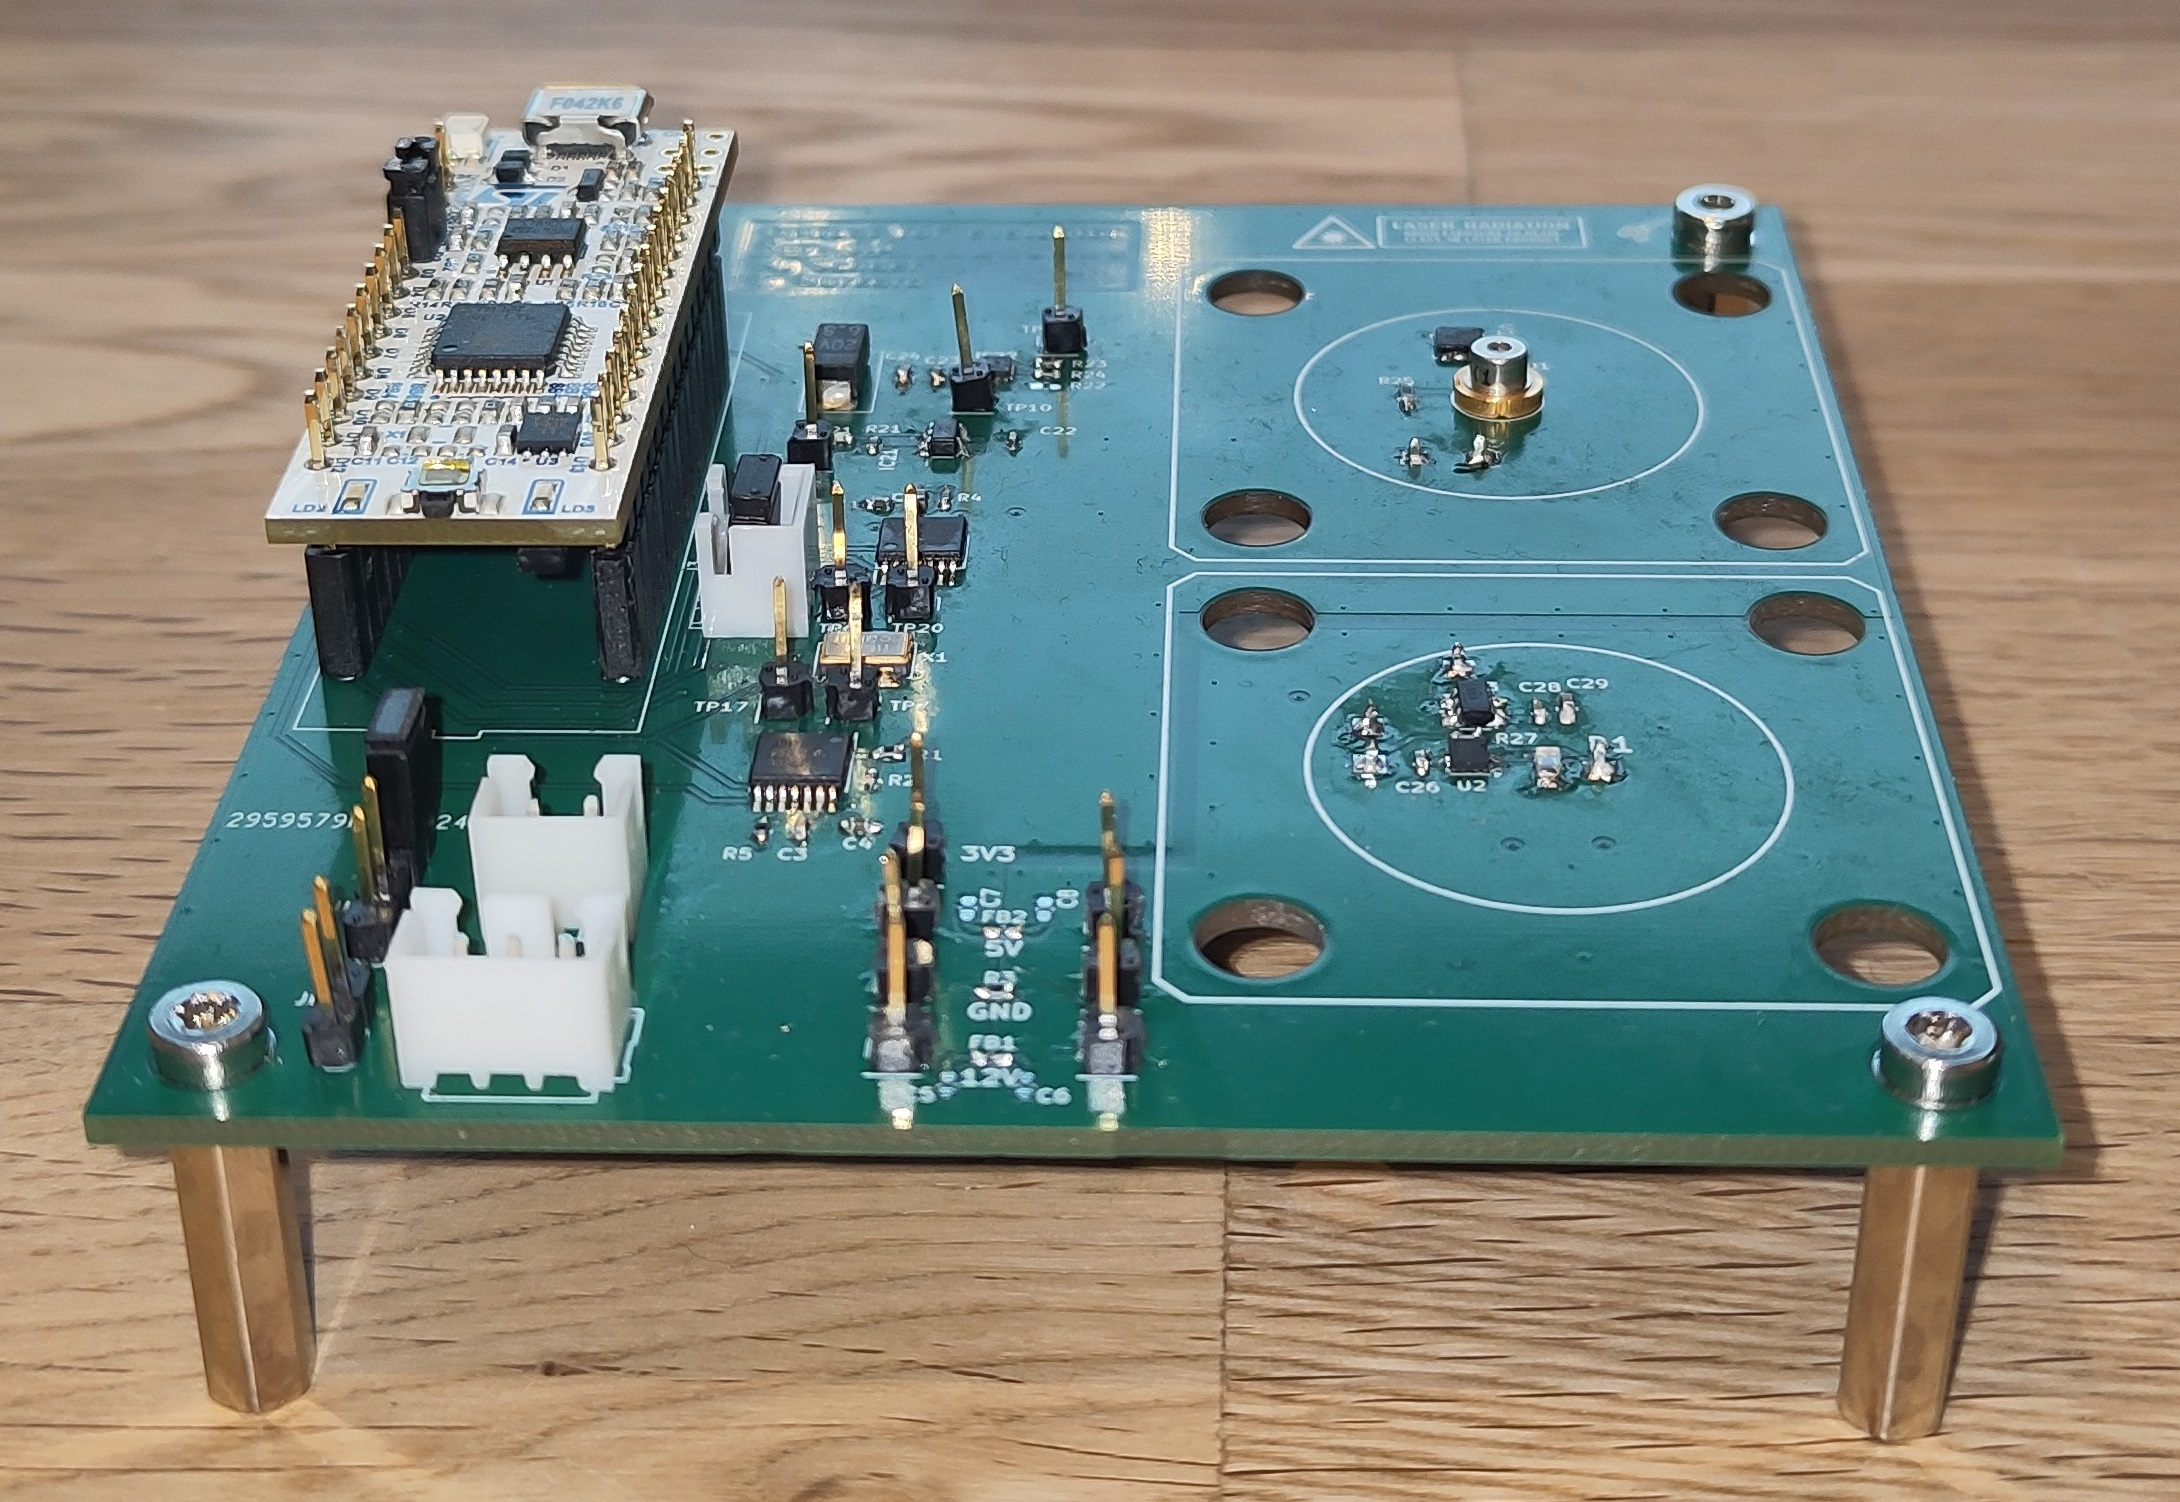
\includegraphics[width=0.6\textwidth]{graphics/photo_demonstrator_front_wo_lens.jpg}
    \caption{Demonstrator von vorne ohne Linse}\label{fig:apdx_photo_demonstrator_front_wo_lens}
\end{figure}

\begin{figure}[H]
    \centering
    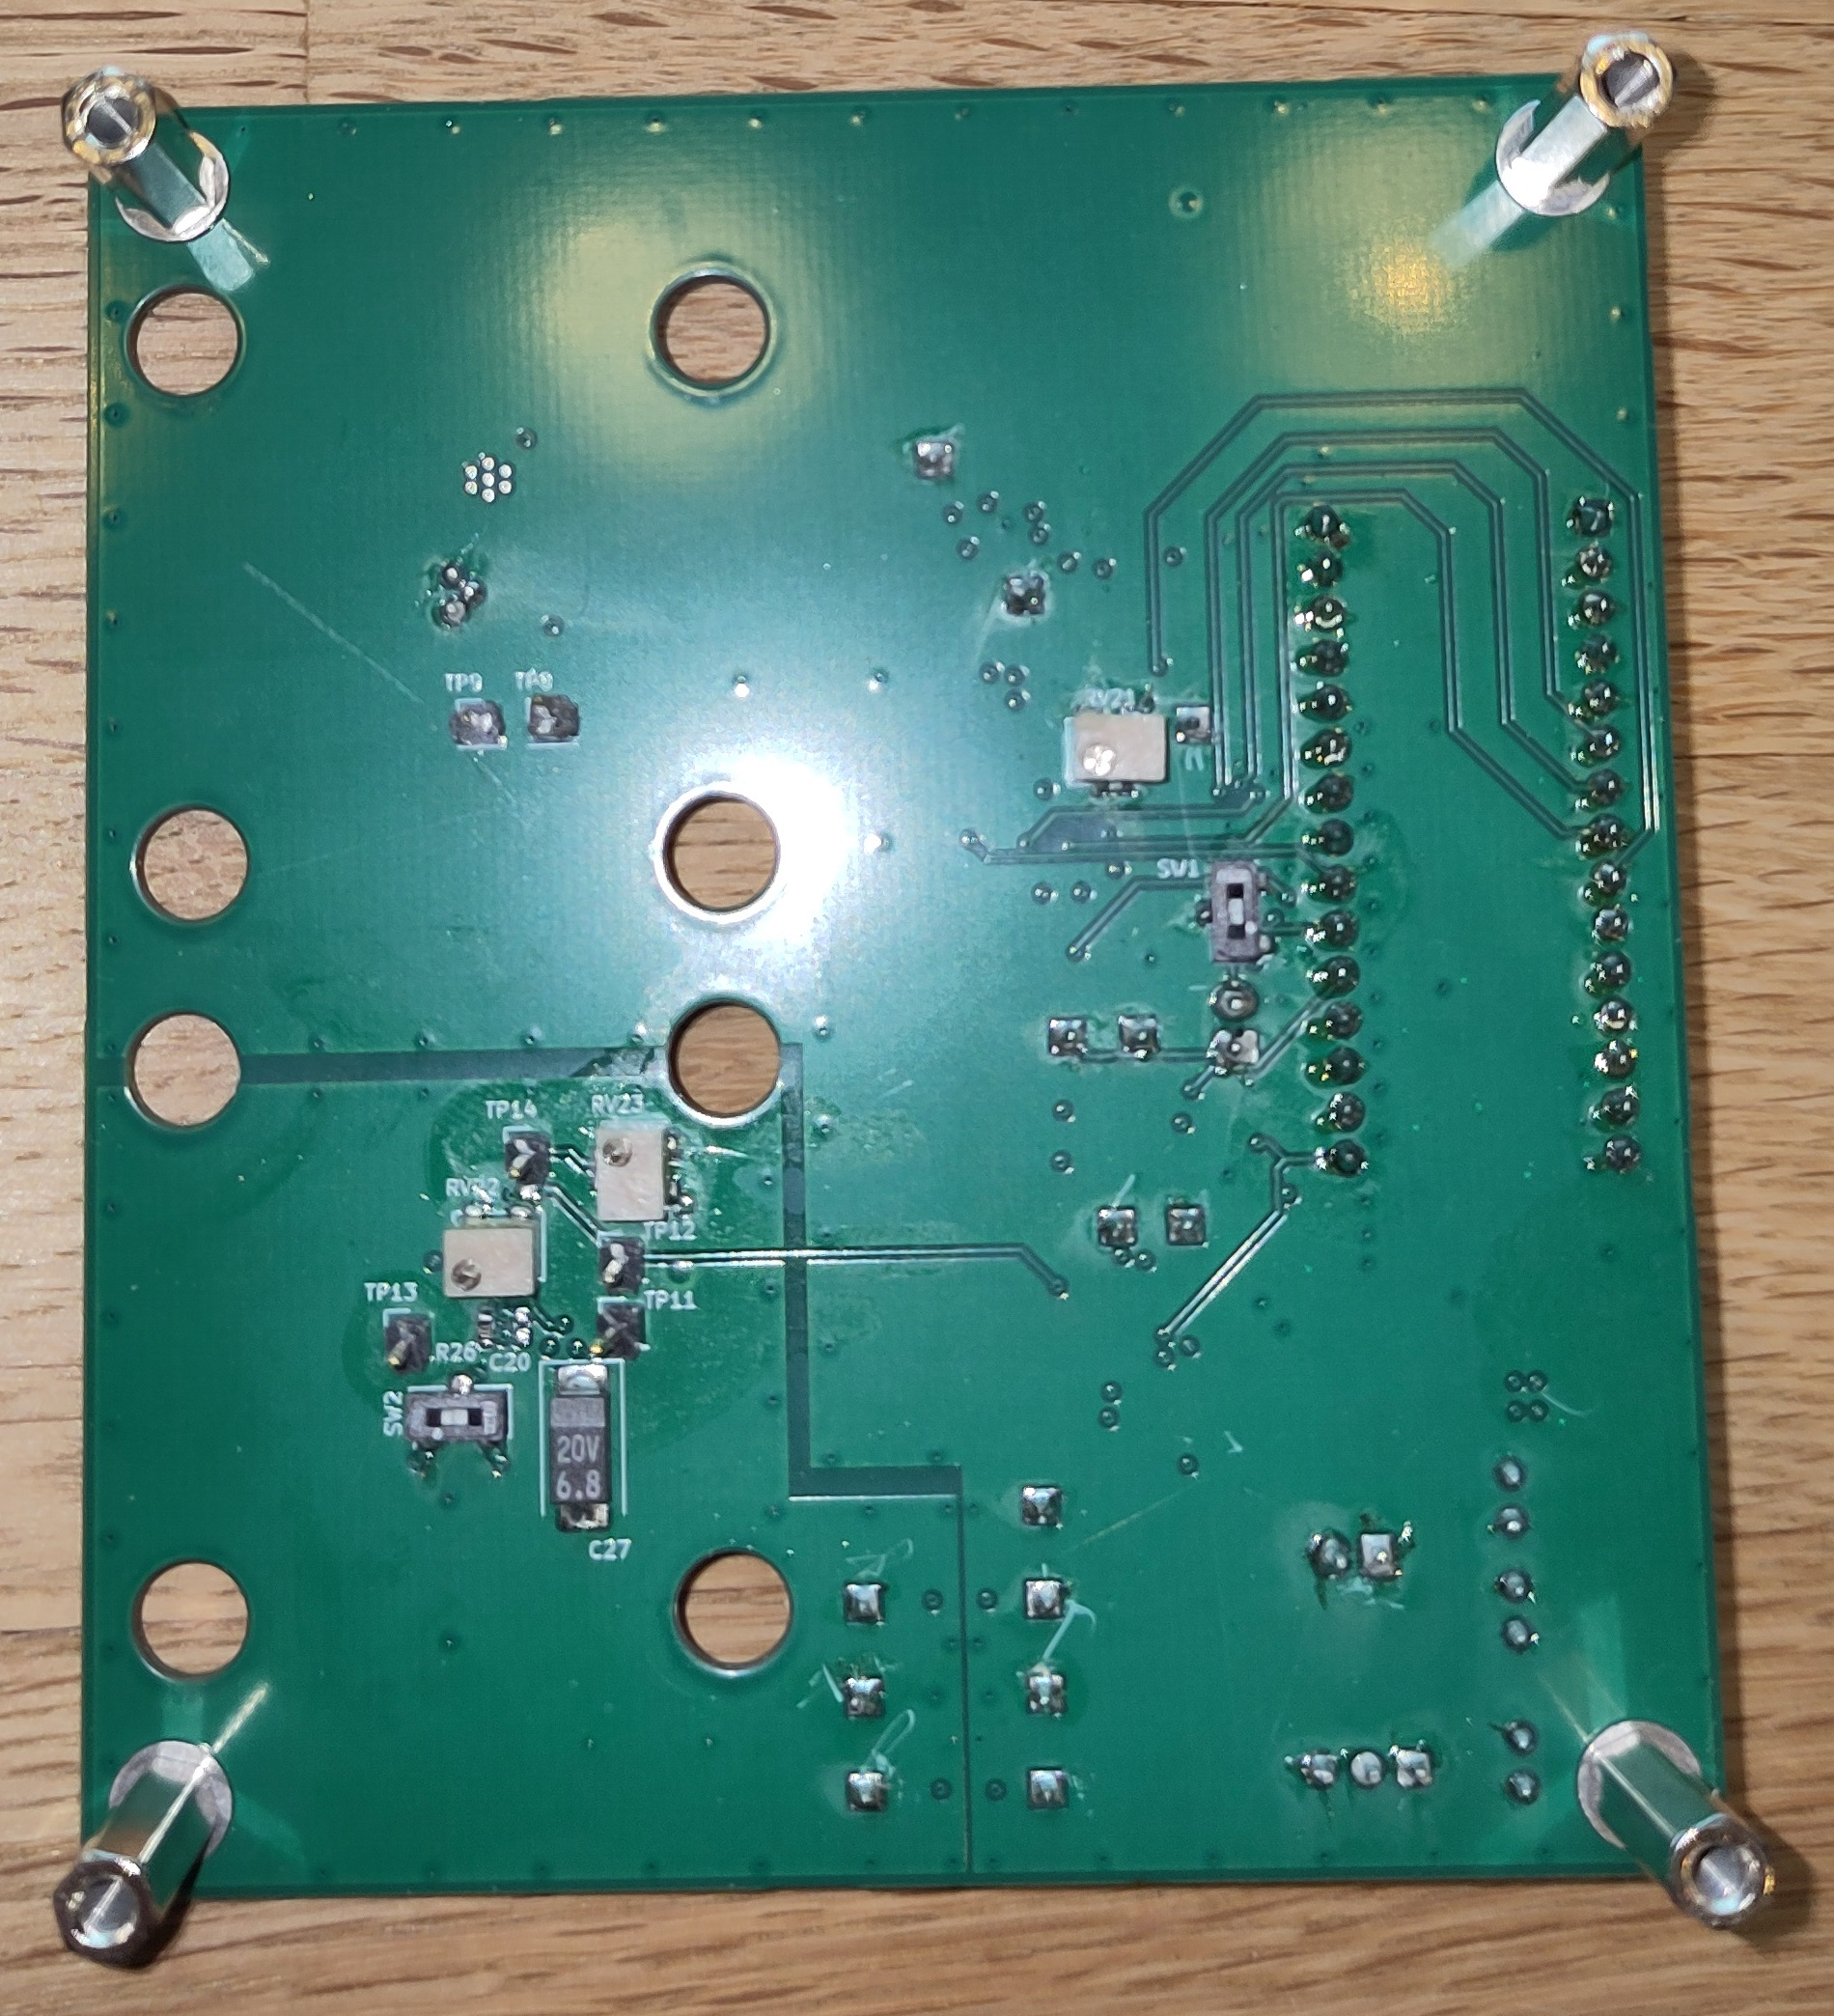
\includegraphics[width=0.6\textwidth]{graphics/photo_demonstrator_bottom.jpg}
    \caption{Demonstrator von unten}\label{fig:apdx_photo_demonstrator_bottom}
\end{figure}
